\documentclass[11pt,fleqn, openany]{book} % Default font size and left-justified equations

%%%%%%%%%%%%%%%%%%%%%%%%%%%%%%%%%%%%%%%%%
% The Legrand Orange Book
% Structural Definitions File
% Version 2.1 (26/09/2018)
%
% Original author:
% Mathias Legrand (legrand.mathias@gmail.com) with modifications by:
% Vel (vel@latextemplates.com)
% 
% This file was downloaded from:
% http://www.LaTeXTemplates.com
%
% License:
% CC BY-NC-SA 3.0 (http://creativecommons.org/licenses/by-nc-sa/3.0/)
%
%%%%%%%%%%%%%%%%%%%%%%%%%%%%%%%%%%%%%%%%%

%----------------------------------------------------------------------------------------
%	VARIOUS REQUIRED PACKAGES AND CONFIGURATIONS
%----------------------------------------------------------------------------------------

\usepackage[table]{xcolor}

\usepackage{graphicx}
\usepackage{tabularx} % Required for including pictures
\usepackage{pgf,tikz,tkz-tab,eurosym,yhmath, stmaryrd}
\usepackage{pgfplots}
\usepackage{mathrsfs}
\usetikzlibrary{patterns}
\usetikzlibrary{trees}
\graphicspath{{../../Pictures/}}
\usepackage{multicol} 


\usepackage[english]{babel} % English language/hyphenation
\usepackage{icomma}
\usepackage{enumitem} % Customize lists
\setlist{nolistsep, nosep, nolistsep} % Reduce spacing between bullet points and numbered lists

\usepackage{booktabs} % Required for nicer horizontal rules in tables

 % Required for specifying colors by name


\definecolor{ocre}{RGB}{243,102,25} % Define the orange color used for highlighting throughout the book

\usepackage{listings}

\definecolor{codegreen}{rgb}{0,0.6,0}
\definecolor{codegray}{rgb}{0.5,0.5,0.5}
\definecolor{codepurple}{rgb}{0.58,0,0.82}
\definecolor{backcolour}{rgb}{0.95,0.95,0.92}

\lstdefinestyle{mystyle}{
    backgroundcolor=\color{backcolour},   
    commentstyle=\color{codegreen},
    keywordstyle=\color{magenta},
    numberstyle=\tiny\color{codegray},
    stringstyle=\color{codepurple},
    basicstyle=\ttfamily\footnotesize,
    breakatwhitespace=false,         
    breaklines=true,                 
    captionpos=b,                    
    keepspaces=true,                 
    numbers=left,                    
    numbersep=5pt,                  
    showspaces=false,                
    showstringspaces=false,
    showtabs=false,                  
    tabsize=2
}

\lstset{style=mystyle}

%----------------------------------------------------------------------------------------
% Paramétrage XSIM
%----------------------------------------------------------------------------------------

\usepackage[no-files]{xsim}


\DeclareExerciseEnvironmentTemplate{myex}{%
    \textbf{%
      \hypertarget{ex:\ExerciseID}{\sffamily{\ensuremath{\blacktriangleright}} Exercice \GetExerciseProperty{counter} \GetExerciseProperty{subtitle} --}
      \hyperlink{sol:\ExerciseID}{Voir le corrigé}%
    }\par
}{\par\smallskip}

\DeclareExerciseEnvironmentTemplate{mysol}{%
    \textbf{%
      \hypertarget{sol:\ExerciseID}{\sffamily{\ensuremath{\blacktriangleright}} Correction \GetExerciseProperty{counter} --}
      \hyperlink{ex:\ExerciseID}{Voir l'énoncé}%
    }\par
}{\par\medskip}

\xsimsetup{
  exercise/template = myex ,
  solution/template = mysol 
}

%Collection exercices

\DeclareExerciseTagging{topic}

\xsimsetup{collect}

%----------------------------------------------------------------------------------------
% SYMBOLES
%----------------------------------------------------------------------------------------

\newcommand\imCMsym[4][\mathord]{%
  \DeclareFontFamily{U} {#2}{}
  \DeclareFontShape{U}{#2}{m}{n}{
    <-6> #25
    <6-7> #26
    <7-8> #27
    <8-9> #28
    <9-10> #29
    <10-12> #210
    <12-> #212}{}
  \DeclareSymbolFont{CM#2} {U} {#2}{m}{n}
  \DeclareMathSymbol{#4}{#1}{CM#2}{#3}
}
\newcommand\alsoimCMsym[4][\mathord]{\DeclareMathSymbol{#4}{#1}{CM#2}{#3}}

\imCMsym{cmmi}{124}{\CMjmath}

\newcommand{\Oij}{(O\,;\,\vec{\imath}\,,\, \vec{\CMjmath} )}
\newcommand{\Oijk}{(O\,;\,\vec{\imath}\,,\, \vec{\CMjmath}\,,\,\vec{k})}

\newcommand\e{\mathrm{e}}
\newcommand\R{\mathbb{R}}
\newcommand\N{\mathbb{N}}


%----------------------------------------------------------------------------------------
%	MARGINS
%----------------------------------------------------------------------------------------

\usepackage{geometry} % Required for adjusting page dimensions and margins

\geometry{
	paper=a4paper, % Paper size, change to letterpaper for US letter size
	top=3cm, % Top margin
	bottom=3cm, % Bottom margin
	left=2cm, % Left margin
	right=2cm, % Right margin
	headheight=14pt, % Header height
	footskip=1.4cm, % Space from the bottom margin to the baseline of the footer
	headsep=10pt, % Space from the top margin to the baseline of the header
	%showframe, % Uncomment to show how the type block is set on the page
}

\setlength{\parindent}{0pt}
\parskip=5pt



%----------------------------------------------------------------------------------------
%	FONTS
%----------------------------------------------------------------------------------------

\usepackage{avant} % Use the Avantgarde font for headings
\usepackage{times} % Use the Times font for headings
\usepackage{mathptmx} % Use the Adobe Times Roman as the default text font together with math symbols from the Sym­bol, Chancery and Com­puter Modern fonts

%\usepackage{microtype} % Slightly tweak font spacing for aesthetics
%\usepackage[utf8]{inputenc} % Required for including letters with accents
\usepackage[T1]{fontenc} % Use 8-bit encoding that has 256 glyphs

%----------------------------------------------------------------------------------------
%	BIBLIOGRAPHY AND INDEX
%----------------------------------------------------------------------------------------

\usepackage[style=numeric,citestyle=numeric,sorting=nyt,sortcites=true,autopunct=true,babel=hyphen,hyperref=true,abbreviate=false,backref=true,backend=biber]{biblatex}
\addbibresource{bibliography.bib} % BibTeX bibliography file
\defbibheading{bibempty}{}

\usepackage{calc} % For simpler calculation - used for spacing the index letter headings correctly
\usepackage{makeidx} % Required to make an index
\makeindex % Tells LaTeX to create the files required for indexing

%----------------------------------------------------------------------------------------
%	MAIN TABLE OF CONTENTS
%----------------------------------------------------------------------------------------

\usepackage{titletoc} % Required for manipulating the table of contents

\contentsmargin{0cm} % Removes the default margin

% Part text styling (this is mostly taken care of in the PART HEADINGS section of this file)
\titlecontents{part}
	[0cm] % Left indentation
	{\addvspace{20pt}\bfseries} % Spacing and font options for parts
	{}
	{}
	{}

% Chapter text styling
\titlecontents{chapter}
	[1.25cm] % Left indentation
	{\addvspace{12pt}\large\sffamily\bfseries} % Spacing and font options for chapters
	{\color{ocre!60}\contentslabel[\Large\thecontentslabel]{1.25cm}\color{ocre}} % Formatting of numbered sections of this type
	{\color{ocre}} % Formatting of numberless sections of this type
	{\color{ocre!60}\normalsize\;\titlerule*[.5pc]{.}\;\thecontentspage} % Formatting of the filler to the right of the heading and the page number

% Section text styling
\titlecontents{section}
	[1.25cm] % Left indentation
	{\addvspace{3pt}\sffamily\bfseries} % Spacing and font options for sections
	{\contentslabel[\thecontentslabel]{1.25cm}} % Formatting of numbered sections of this type
	{} % Formatting of numberless sections of this type
	{\hfill\color{black}\thecontentspage} % Formatting of the filler to the right of the heading and the page number

% Subsection text styling
\titlecontents{subsection}
	[1.25cm] % Left indentation
	{\addvspace{1pt}\sffamily\small} % Spacing and font options for subsections
	{\contentslabel[\thecontentslabel]{1.25cm}} % Formatting of numbered sections of this type
	{} % Formatting of numberless sections of this type
	{\ \titlerule*[.5pc]{.}\;\thecontentspage} % Formatting of the filler to the right of the heading and the page number

% Figure text styling
\titlecontents{figure}
	[1.25cm] % Left indentation
	{\addvspace{1pt}\sffamily\small} % Spacing and font options for figures
	{\thecontentslabel\hspace*{1em}} % Formatting of numbered sections of this type
	{} % Formatting of numberless sections of this type
	{\ \titlerule*[.5pc]{.}\;\thecontentspage} % Formatting of the filler to the right of the heading and the page number

% Table text styling
\titlecontents{table}
	[1.25cm] % Left indentation
	{\addvspace{1pt}\sffamily\small} % Spacing and font options for tables
	{\thecontentslabel\hspace*{1em}} % Formatting of numbered sections of this type
	{} % Formatting of numberless sections of this type
	{\ \titlerule*[.5pc]{.}\;\thecontentspage} % Formatting of the filler to the right of the heading and the page number

%----------------------------------------------------------------------------------------
%	MINI TABLE OF CONTENTS IN PART HEADS
%----------------------------------------------------------------------------------------

% Chapter text styling
\titlecontents{lchapter}
	[0em] % Left indentation
	{\addvspace{15pt}\large\sffamily\bfseries} % Spacing and font options for chapters
	{\color{ocre}\contentslabel[\Large\thecontentslabel]{1.25cm}\color{ocre}} % Chapter number
	{}  
	{\color{ocre}\normalsize\sffamily\bfseries\;\titlerule*[.5pc]{.}\;\thecontentspage} % Page number

% Section text styling
\titlecontents{lsection}
	[0em] % Left indentation
	{\sffamily\small} % Spacing and font options for sections
	{\contentslabel[\thecontentslabel]{1.25cm}} % Section number
	{}
	{}

% Subsection text styling (note these aren't shown by default, display them by searchings this file for tocdepth and reading the commented text)
\titlecontents{lsubsection}
	[.5em] % Left indentation
	{\sffamily\footnotesize} % Spacing and font options for subsections
	{\contentslabel[\thecontentslabel]{1.25cm}}
	{}
	{}

%----------------------------------------------------------------------------------------
%	HEADERS AND FOOTERS
%----------------------------------------------------------------------------------------


\usepackage{fancyhdr} % Required for header and footer configuration

\pagestyle{fancy}
\renewcommand{\chaptermark}[1]{\markboth{\sffamily\normalsize\bfseries\ \thechapter.\ #1}{}} % Chapter text font settings
\renewcommand{\sectionmark}[1]{\markright{\sffamily\normalsize\thesection\hspace{5pt}#1}{}} % Section text font settings
\fancyhf{} \fancyhead[LE,RO]{\sffamily\normalsize\thepage} % Font setting for the page number in the header
\fancyhead[LO]{\rightmark} % Print the nearest section name on the left side of odd pages
\fancyhead[RE]{\leftmark} % Print the current chapter name on the right side of even pages

\fancyfoot[L]{Jason LAPEYRONNIE}
\fancyfoot[R]{\href{http://mathoutils.fr}{http://mathoutils.fr}} % Uncomment to include a footer

\renewcommand{\headrulewidth}{0.5pt} % Thickness of the rule under the header
\renewcommand{\footrulewidth}{0.5pt} % Thickness of the rule under the header

\fancypagestyle{plain}{% Style for when a plain pagestyle is specified
	\fancyhead{}\renewcommand{\headrulewidth}{0pt}%
}

% Removes the header from odd empty pages at the end of chapters
\makeatletter
\renewcommand{\cleardoublepage}{
\clearpage\ifodd\c@page\else
\hbox{}
\vspace*{\fill}
\thispagestyle{empty}
\newpage
\fi}

%----------------------------------------------------------------------------------------
%	THEOREM STYLES
%----------------------------------------------------------------------------------------

\usepackage{amsmath,amsfonts,amssymb,amsthm} % For math equations, theorems, symbols, etc

\newcommand{\intoo}[2]{\mathopen{]}#1\,;#2\mathclose{[}}
\newcommand{\ud}{\mathop{\mathrm{{}d}}\mathopen{}}
\newcommand{\intff}[2]{\mathopen{[}#1\,;#2\mathclose{]}}
\renewcommand{\qedsymbol}{$\blacksquare$}
\newtheorem{notation}{Notation}[section]

% Boxed/framed environments
\newtheoremstyle{ocrenumbox}% Theorem style name
{0pt}% Space above
{0pt}% Space below
{\normalfont}% Body font
{}% Indent amount
{\small\bf\sffamily\color{ocre}}% Theorem head font
{\;:\;}% Punctuation after theorem head
{0.25em}% Space after theorem head
{\small\sffamily\color{ocre}\thmname{#1}\nobreakspace\thmnumber{\@ifnotempty{#1}{}\@upn{#2}}% Theorem text (e.g. Theorem 2.1)
\thmnote{\nobreakspace\the\thm@notefont\sffamily\bfseries\color{black}---\nobreakspace#3}} % Optional theorem note

\newtheoremstyle{blacknumex}% Theorem style name
{5pt}% Space above
{10pt}% Space below
{\normalfont}% Body font
{} % Indent amount
{\small\bf\sffamily}% Theorem head font
{\;:\;}% Punctuation after theorem head
{0.25em}% Space after theorem head
{\small\sffamily{\tiny\ensuremath{\blacksquare}}\nobreakspace\thmname{#1}\nobreakspace\thmnumber{\@ifnotempty{#1}{}\@upn{#2}}% Theorem text (e.g. Theorem 2.1)
\thmnote{\nobreakspace\the\thm@notefont\sffamily\bfseries---\nobreakspace#3}}% Optional theorem note

\newtheoremstyle{blacknumexo}% Theorem style name
{15pt}% Space above
{10pt}% Space below
{\normalfont}% Body font
{} % Indent amount
{\small\bf\sffamily}% Theorem head font
{}% Punctuation after theorem head
{0.5em}% Space after theorem head
{\small\sffamily{\ensuremath{\blacktriangleright}}\nobreakspace\thmname{#1}\nobreakspace\thmnumber{\@ifnotempty{#1}{}\@upn{#2}}% Theorem text (e.g. Theorem 2.1)
\thmnote{\nobreakspace\the\thm@notefont\sffamily\bfseries---\nobreakspace#3} \\}% Optional theorem note



\newtheoremstyle{blacknumbox} % Theorem style name
{0pt}% Space above
{5pt}% Space below
{}% Body font
{}% Indent amount
{\large\bf\sffamily}% Theorem head font
{\;:\;}% Punctuation after theorem head
{0.25em}% Space after theorem head
{\small\sffamily\thmname{#1}\nobreakspace\thmnumber{\@ifnotempty{#1}{}\@upn{#2}}% Theorem text (e.g. Theorem 2.1)
\thmnote{\nobreakspace\the\thm@notefont\sffamily\bfseries---\nobreakspace#3}}% Optional theorem note

% Non-boxed/non-framed environments
\newtheoremstyle{ocrenum}% Theorem style name
{5pt}% Space above
{5pt}% Space below
{\normalfont}% Body font
{}% Indent amount
{\small\bf\sffamily\color{ocre}}% Theorem head font
{\;:\;}% Punctuation after theorem head
{0.25em}% Space after theorem head
{\small\sffamily\color{ocre}\thmname{#1}\nobreakspace\thmnumber{\@ifnotempty{#1}{}\@upn{#2}}% Theorem text (e.g. Theorem 2.1)
\thmnote{\nobreakspace\the\thm@notefont\sffamily\bfseries\color{black}---\nobreakspace#3}} % Optional theorem note
\makeatother

% Defines the theorem text style for each type of theorem to one of the three styles above
\newcounter{dummy} 
\newcounter{thm}
\newcounter{correction}
\newcounter{qst}
\theoremstyle{ocrenumbox}
\newtheorem{theoremeT}[dummy]{Théorème}
\newtheorem{exerciseT}{Propriété}
\newtheorem{principeT}{Principe}
\theoremstyle{blacknumex}
\newtheorem{exampleT}{Exemple}
\theoremstyle{blacknumexo}
\newtheorem{exo}[thm]{Exercice}
\newtheorem{corr}[correction]{Correction}
\newtheorem{quest}[qst]{Question}
\theoremstyle{blacknumbox}
\newtheorem{vocabulary}{Vocabulary}[section]
\newtheorem{definitionT}{Définition}
\newtheorem{corollaryT}[dummy]{Corollary}
\theoremstyle{ocrenum}
\newtheorem{proofT}[dummy]{Démonstration}


%----------------------------------------------------------------------------------------
%	DEFINITION OF COLORED BOXES
%----------------------------------------------------------------------------------------

\RequirePackage[framemethod=default]{mdframed} % Required for creating the theorem, definition, exercise and corollary boxes

% Theorem box
\newmdenv[skipabove=7pt,
skipbelow=7pt,
backgroundcolor=black!5,
linecolor=ocre,
innerleftmargin=5pt,
innerrightmargin=5pt,
innertopmargin=10pt,
leftmargin=0cm,
rightmargin=0cm,
innerbottommargin=5pt]{tBox}

%Proposition box	  
\newmdenv[skipabove=7pt,
skipbelow=7pt,
rightline=false,
leftline=true,
topline=false,
bottomline=false,
backgroundcolor=ocre!10,
linecolor=ocre,
innerleftmargin=5pt,
innerrightmargin=5pt,
innertopmargin=10pt,
innerbottommargin=3pt,
leftmargin=0cm,
rightmargin=0cm,
linewidth=4pt]{eBox}	

% Definition box
\newmdenv[skipabove=7pt,
backgroundcolor=ocre!4,
skipbelow=7pt,
rightline=false,
leftline=true,
topline=false,
bottomline=false,
linecolor=ocre,
innerleftmargin=5pt,
innerrightmargin=5pt,
innertopmargin=10pt,
leftmargin=0cm,
rightmargin=0cm,
linewidth=4pt,
innerbottommargin=5pt]{dBox}	

% Corollary box
\newmdenv[skipabove=7pt,
skipbelow=7pt,
rightline=false,
leftline=true,
topline=false,
bottomline=false,
linecolor=gray,
backgroundcolor=black!5,
innerleftmargin=5pt,
innerrightmargin=5pt,
innertopmargin=5pt,
leftmargin=0cm,
rightmargin=0cm,
linewidth=4pt,
innerbottommargin=5pt]{cBox}

\newmdenv[skipabove=7pt,
skipbelow=7pt,
backgroundcolor=black!5,
innerleftmargin=5pt,
topline=false,
bottomline=false,
rightline=false,
leftline=false,
innerrightmargin=5pt,
innertopmargin=5pt,
leftmargin=0cm,
rightmargin=0cm,
innerbottommargin=5pt]{xBox}

% Creates an environment for each type of theorem and assigns it a theorem text style from the "Theorem Styles" section above and a colored box from above
\newenvironment{theorem}{\begin{tBox}\begin{theoremeT}}{\end{theoremeT}\end{tBox}}

\newenvironment{exo2}{\noindent \begin{exo}\item\relax \noindent \begin{eBox}\item\relax}{\end{eBox}\end{exo}}


\newenvironment{proposition}{\begin{eBox}\begin{exerciseT}}{\hfill{\color{ocre}}\end{exerciseT}\end{eBox}}		

\newenvironment{principe}{\begin{eBox}\begin{principeT}}{\hfill{\color{ocre}}\end{principeT}\end{eBox}}	
		  
\newenvironment{definition}{\begin{dBox}\begin{definitionT}}{\end{definitionT}\end{dBox}}	

\newenvironment{example}{\begin{xBox}\begin{exampleT}}{\hfill{\tiny\ensuremath{\blacksquare}}\end{exampleT}\end{xBox}}

\newenvironment{demonstration}{\begin{proofT}}{\hfill{\tiny\ensuremath{\square}}\end{proofT}}		
\newenvironment{corollary}{\begin{cBox}\begin{corollaryT}}{\end{corollaryT}\end{cBox}}	

%----------------------------------------------------------------------------------------
%	REMARK ENVIRONMENT
%----------------------------------------------------------------------------------------

\newenvironment{remark}{\par\vspace{5pt}\small % Vertical white space above the remark and smaller font size
\begin{list}{}{
\leftmargin=25pt % Indentation on the left
\rightmargin=15pt}\item\ignorespaces % Indentation on the right
\makebox[-2.5pt]{
\begin{tikzpicture}[overlay]
\node[draw=ocre!60,line width=1pt,circle,fill=ocre!25,font=\sffamily\bfseries,inner sep=2pt,outer sep=0pt] at (-15pt,0pt){\textcolor{ocre}{R}};\end{tikzpicture}} % Orange R in a circle
\advance\baselineskip -1pt}{\end{list}\vskip5pt} % Tighter line spacing and white space after remark

%----------------------------------------------------------------------------------------
%	SECTION NUMBERING IN THE MARGIN
%----------------------------------------------------------------------------------------

\makeatletter
\renewcommand{\@seccntformat}[1]{\llap{\textcolor{ocre}{\csname the#1\endcsname}\hspace{1em}}}                    
\renewcommand{\section}{\@startsection{section}{1}{\z@}
{-4ex \@plus -1ex \@minus -.4ex}
{1ex \@plus.2ex }
{\normalfont\LARGE\sffamily\bfseries}}
\renewcommand{\subsection}{\@startsection {subsection}{2}{\z@}
{-3ex \@plus -0.1ex \@minus -.4ex}
{0.5ex \@plus.2ex }
{\normalfont\sffamily\bfseries}}
\renewcommand{\subsubsection}{\@startsection {subsubsection}{3}{\z@}
{-2ex \@plus -0.1ex \@minus -.2ex}
{.2ex \@plus.2ex }
{\normalfont\small\sffamily\bfseries}}                        
\renewcommand\paragraph{\@startsection{paragraph}{4}{\z@}
{-2ex \@plus-.2ex \@minus .2ex}
{.1ex}
{\normalfont\small\sffamily\bfseries}}

%----------------------------------------------------------------------------------------
%	PART HEADINGS
%----------------------------------------------------------------------------------------

% Numbered part in the table of contents
\newcommand{\@mypartnumtocformat}[2]{%
	\setlength\fboxsep{0pt}%
	\noindent\colorbox{ocre!20}{\strut\parbox[c][.7cm]{\ecart}{\color{ocre!70}\Large\sffamily\bfseries\centering#1}}\hskip\esp\colorbox{ocre!40}{\strut\parbox[c][.7cm]{\linewidth-\ecart-\esp}{\Large\sffamily\centering#2}}%
}

% Unnumbered part in the table of contents
\newcommand{\@myparttocformat}[1]{%
	\setlength\fboxsep{0pt}%
	\noindent\colorbox{ocre!40}{\strut\parbox[c][.7cm]{\linewidth}{\Large\sffamily\centering#1}}%
}

\newlength\esp
\setlength\esp{4pt}
\newlength\ecart
\setlength\ecart{1.2cm-\esp}
\newcommand{\thepartimage}{}%
\newcommand{\partimage}[1]{\renewcommand{\thepartimage}{#1}}%
\def\@part[#1]#2{%
\ifnum \c@secnumdepth >-2\relax%
\refstepcounter{part}%
\addcontentsline{toc}{part}{\texorpdfstring{\protect\@mypartnumtocformat{\thepart}{#1}}{\partname~\thepart\ ---\ #1}}
\else%
\addcontentsline{toc}{part}{\texorpdfstring{\protect\@myparttocformat{#1}}{#1}}%
\fi%
\startcontents%
\markboth{}{}%
{\thispagestyle{empty}%
\begin{tikzpicture}[remember picture,overlay]%
\node at (current page.north west){\begin{tikzpicture}[remember picture,overlay]%	
\fill[ocre!20](0cm,0cm) rectangle (\paperwidth,-\paperheight);
\node[anchor=north] at (4cm,-3.25cm){\color{ocre!40}\fontsize{220}{100}\sffamily\bfseries\thepart}; 
\node[anchor=south east] at (\paperwidth-1cm,-\paperheight+1cm){\parbox[t][][t]{8.5cm}{
\printcontents{l}{0}{\setcounter{tocdepth}{1}}% The depth to which the Part mini table of contents displays headings; 0 for chapters only, 1 for chapters and sections and 2 for chapters, sections and subsections
}};
\node[anchor=north east] at (\paperwidth-1.5cm,-3.25cm){\parbox[t][][t]{15cm}{\strut\raggedleft\color{white}\fontsize{30}{30}\sffamily\bfseries#2}};
\end{tikzpicture}};
\end{tikzpicture}}%
\@endpart}
\def\@spart#1{%
\startcontents%
\phantomsection
{\thispagestyle{empty}%
\begin{tikzpicture}[remember picture,overlay]%
\node at (current page.north west){\begin{tikzpicture}[remember picture,overlay]%	
\fill[ocre!20](0cm,0cm) rectangle (\paperwidth,-\paperheight);
\node[anchor=north east] at (\paperwidth-1.5cm,-3.25cm){\parbox[t][][t]{15cm}{\strut\raggedleft\color{white}\fontsize{30}{30}\sffamily\bfseries#1}};
\end{tikzpicture}};
\end{tikzpicture}}
\addcontentsline{toc}{part}{\texorpdfstring{%
\setlength\fboxsep{0pt}%
\noindent\protect\colorbox{ocre!40}{\strut\protect\parbox[c][.7cm]{\linewidth}{\Large\sffamily\protect\centering #1\quad\mbox{}}}}{#1}}%
\@endpart}
\def\@endpart{\vfil\newpage
\if@twoside
\if@openright
\null
\thispagestyle{empty}%
\newpage
\fi
\fi
\if@tempswa
\twocolumn
\fi}

%----------------------------------------------------------------------------------------
%	CHAPTER HEADINGS
%----------------------------------------------------------------------------------------

% A switch to conditionally include a picture, implemented by Christian Hupfer
\newif\ifusechapterimage
\usechapterimagetrue
\newcommand{\thechapterimage}{}%
\newcommand{\chapterimage}[1]{\ifusechapterimage\renewcommand{\thechapterimage}{#1}\fi}%
\newcommand{\autodot}{.}
\def\@makechapterhead#1{%
{\parindent \z@ \raggedright \normalfont
\ifnum \c@secnumdepth >\m@ne
\if@mainmatter
\begin{tikzpicture}[remember picture,overlay]
\node at (current page.north west)
{\begin{tikzpicture}[remember picture,overlay]
\node[anchor=north west,inner sep=0pt] at (0,0) {\ifusechapterimage\includegraphics[width=\paperwidth]{\thechapterimage}\fi};
\draw[anchor=west] (\Gm@lmargin,-3cm) node [line width=2pt,rounded corners=15pt,draw=ocre,fill=white,fill opacity=0.5,inner sep=15pt]{\strut\makebox[22cm]{}};
\draw[anchor=west] (\Gm@lmargin+.3cm,-3cm) node {\huge\sffamily\bfseries\color{black}\thechapter\autodot~#1\strut};
\end{tikzpicture}};
\end{tikzpicture}
\else
\begin{tikzpicture}[remember picture,overlay]
\node at (current page.north west)
{\begin{tikzpicture}[remember picture,overlay]
\node[anchor=north west,inner sep=0pt] at (0,0) {\ifusechapterimage\includegraphics[width=\paperwidth]{\thechapterimage}\fi};
\draw[anchor=west] (\Gm@lmargin,-3cm) node [line width=2pt,rounded corners=15pt,draw=ocre,fill=white,fill opacity=0.5,inner sep=15pt]{\strut\makebox[22cm]{}};
\draw[anchor=west] (\Gm@lmargin+.3cm,-3cm) node {\huge\sffamily\bfseries\color{black}#1\strut};
\end{tikzpicture}};
\end{tikzpicture}
\fi\fi\par\vspace*{50\p@}}}

%-------------------------------------------

\def\@makeschapterhead#1{%
\begin{tikzpicture}[remember picture,overlay]
\node at (current page.north west)
{\begin{tikzpicture}[remember picture,overlay]
\node[anchor=north west,inner sep=0pt] at (0,0) {\ifusechapterimage\includegraphics[width=\paperwidth]{\thechapterimage}\fi};
\draw[anchor=west] (\Gm@lmargin,-3cm) node [line width=2pt,rounded corners=15pt,draw=ocre,fill=white,fill opacity=0.5,inner sep=15pt]{\strut\makebox[22cm]{}};
\draw[anchor=west] (\Gm@lmargin+.3cm,-3cm) node {\huge\sffamily\bfseries\color{black}#1\strut};
\end{tikzpicture}};
\end{tikzpicture}
\par\vspace*{50\p@}}
\makeatother

%----------------------------------------------------------------------------------------
%	LINKS
%----------------------------------------------------------------------------------------

\usepackage{hyperref}
\hypersetup{hidelinks,backref=true,pagebackref=true,hyperindex=true,colorlinks=false,breaklinks=true,urlcolor=ocre,bookmarks=true,bookmarksopen=false}

\usepackage{bookmark}
\bookmarksetup{
open,
numbered,
addtohook={%
\ifnum\bookmarkget{level}=0 % chapter
\bookmarksetup{bold}%
\fi
\ifnum\bookmarkget{level}=-1 % part
\bookmarksetup{color=ocre,bold}%
\fi
}
}

\renewcommand*\thesection{\arabic{section}}

\newcommand*{\coord}[3]{% 
  \ensuremath{\overrightarrow{#1}\, 
    \begin{pmatrix} 
      #2\\ 
      #3 
    \end{pmatrix}}}
    
  \newcommand*{\coordb}[2]{% 
  \ensuremath{ 
    \begin{pmatrix} 
      #1\\ 
      #2 
    \end{pmatrix}}}

\newcommand*{\coorde}[4]{% 
  \renewcommand{\arraystretch}{1}\ensuremath{\overrightarrow{#1}\, 
    \begin{pmatrix} 
      #2\\ 
      #3 \\
      #4
    \end{pmatrix}}}    
  \newcommand*{\coordbe}[3]{% 
 \renewcommand{\arraystretch}{1} \ensuremath{ 
    \begin{pmatrix} 
      #1\\ 
      #2 \\
      #3
    \end{pmatrix}}}  
    
\newcommand{\Card}{\mathrm{Card}}


\begin{document}

\chapterimage{../../Pictures/background}

\chapter{Exercices}

\section*{Rappels}

\begin{exercise} On se place sur le cercle trigonométrique tracé ci-dessus et sur lequel sont placés certains points.

\begin{minipage}{0.5\linewidth}

\begin{center}
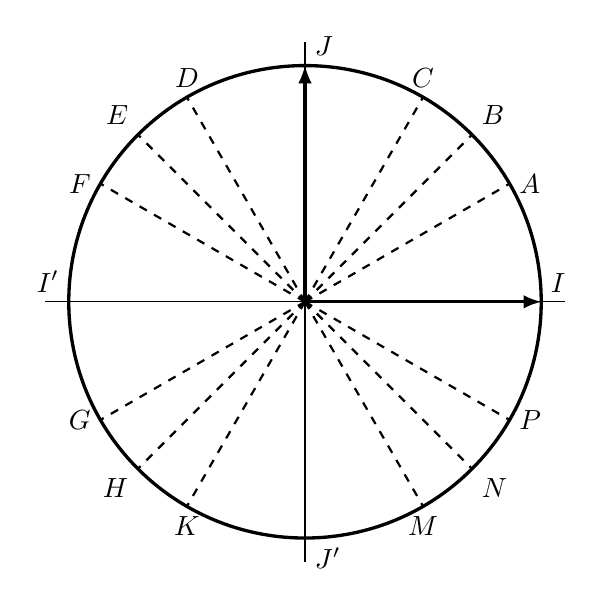
\begin{tikzpicture}[scale=3]
\draw [very thick,>=latex,->] (0,0) -- (0,1);
\draw [very thick,>=latex,->] (0,0) -- (1,0);
\draw (-1.1,0) -- (1.1,0);
\draw (0,1.1) -- (0,-1.1);
\draw [very thick] (1,0) arc (0:360:1);
\draw [thick, dashed] (0:0) -- (30:1);
\draw [thick, dashed] (0:0) -- (45:1);
\draw [thick, dashed] (0:0) -- (60:1);
\draw [thick, dashed] (0:0) -- (120:1);
\draw [thick, dashed] (0:0) -- (135:1);
\draw [thick, dashed] (0:0) -- (150:1);
\draw [thick, dashed] (0:0) -- (-30:1);
\draw [thick, dashed] (0:0) -- (-45:1);
\draw [thick, dashed] (0:0) -- (-60:1);
\draw [thick, dashed] (0:0) -- (-120:1);
\draw [thick, dashed] (0:0) -- (-135:1);
\draw [thick, dashed] (0:0) -- (-150:1);
\draw (30:1) node[right] {$A$};
\draw (45:1) node[above right] {$B$};
\draw (60:1) node[above] {$C$};
\draw (90:1) node[above right] {$J$};
\draw (180:1) node[above left] {$I'$};
\draw (0:1) node[above right] {$I$};
\draw (120:1) node[above] {$D$};
\draw (135:1) node[above left] {$E$};
\draw (150:1) node[left] {$F$};
\draw (-30:1) node[right] {$P$};
\draw (-45:1) node[below right] {$N$};
\draw (-60:1) node[below] {$M$};
\draw (-90:1) node[below right] {$J'$};
\draw (-120:1) node[below] {$K$};
\draw (-135:1) node[below left] {$H$};
\draw (-150:1) node[left] {$G$};
\end{tikzpicture}
\end{center}
\end{minipage}\hfill\begin{minipage}{0.45\linewidth}
Déterminer les points images par l'enroulement de la droite des réels sur le cercle trigonométrique des réels suivants.
\renewcommand{\arraystretch}{2.5}
\begin{tabularx}{\linewidth}{XXXX}
$\pi$ & $2\pi$ & $-3\pi$ & $18\pi$ \\
$\dfrac{\pi}{2}$ & $\dfrac{3\pi}{2}$ & $\dfrac{17\pi}{2}$ & $\dfrac{-7\pi}{2}$\\
$\dfrac{\pi}{6}$ & $\dfrac{3\pi}{4}$ & $\dfrac{-5\pi}{3}$ & $\dfrac{8\pi}{3}$ \\
$\dfrac{-7\pi}{4}$ & $\dfrac{19\pi}{3}$ & $\dfrac{-37\pi}{6}$ & $\dfrac{23\pi}{4}$\end{tabularx}
\end{minipage}\end{exercise}

\begin{solution}

\renewcommand{\arraystretch}{2}\begin{tabularx}{\linewidth}{XXXX}
$\pi$ : $I'$ & $2\pi$ : $I$ & $-3\pi$ : $I'$ & $18\pi$ : $I$ \\
$\dfrac{\pi}{2}$ : $J$& $\dfrac{3\pi}{2}$ : $J'$ & $\dfrac{17\pi}{2}$ : $J$ & $\dfrac{-7\pi}{2}$ : $J$\\
$\dfrac{\pi}{6}$ : $A$& $\dfrac{3\pi}{4}$ : $E$ & $\dfrac{-5\pi}{3}$ : $C$ & $\dfrac{8\pi}{3}$ : $D$\\
$\dfrac{-7\pi}{4}$ : $B$ & $\dfrac{19\pi}{3}$ : $C$ & $\dfrac{-37\pi}{6}$ : $P$ & $\dfrac{23\pi}{4}$ : $N$\end{tabularx}

\end{solution}



\begin{exercise} En utilisant le cercle trigonométrique, déterminer les valeurs suivantes.

\begin{tabularx}{\linewidth}{XXXX}
$\cos \left( -\dfrac{\pi}{3} \right)$ & $\sin \left(- \dfrac{\pi}{3} \right)$ & $\cos \left( \dfrac{2\pi}{3} \right)$ & $\sin \left( \dfrac{2\pi}{3} \right)$ \\
$\cos \left( -\dfrac{\pi}{4} \right)$ & $\sin \left( \dfrac{5\pi}{4} \right)$ & $\cos \left( \dfrac{3\pi}{4} \right)$ & $\sin \left( \dfrac{3\pi}{4} \right)$ \\
$\cos \left( \dfrac{11\pi}{6} \right)$ & $\sin \left(- \dfrac{5\pi}{6} \right)$ & $\cos \left( \dfrac{5\pi}{6} \right)$ & $\sin \left( -\dfrac{\pi}{6} \right)$ 
\end{tabularx}\end{exercise}


\begin{solution}

\begin{tabularx}{\linewidth}{XXXX}
$\cos \left( -\dfrac{\pi}{3} \right) = \dfrac{1}{2}$ & $\sin \left(- \dfrac{\pi}{3} \right)=-\dfrac{\sqrt{3}}{2}$ & $\cos \left( \dfrac{2\pi}{3} \right) = -\dfrac{1}{2}$ & $\sin \left( \dfrac{2\pi}{3} \right) = \dfrac{\sqrt{3}}{2}$ \\
$\cos \left( -\dfrac{\pi}{4} \right) = -\dfrac{\sqrt{2}}{2}$ & $\sin \left( \dfrac{5\pi}{4} \right)=-\dfrac{\sqrt{2}}{2}$ & $\cos \left( \dfrac{3\pi}{4} \right)=-\dfrac{\sqrt{2}}{2}$ & $\sin \left( \dfrac{3\pi}{4} \right) = \dfrac{\sqrt{2}}{2}$ \\
$\cos \left( \dfrac{11\pi}{6} \right)=\dfrac{\sqrt{3}}{2}$ & $\sin \left(- \dfrac{5\pi}{6} \right)=-\dfrac{1}{2}$ & $\cos \left( \dfrac{5\pi}{6} \right)=-\dfrac{\sqrt{3}}{2}$ & $\sin \left( -\dfrac{\pi}{6} \right)=-\dfrac{1}{2}$ 
\end{tabularx}\end{solution}



\begin{exercise}Résoudre les équations suivantes, d'inconnue $x\in]-\pi;\pi]$.

\begin{tabularx}{\linewidth}{XXXX}
$\cos (x)=\dfrac{1}{2}$ & $\sin (x) = \dfrac{\sqrt{2}}{2}$ & $\cos (x)=0$ & $\sin (x)=-\dfrac{\sqrt{3}}{2}$
\end{tabularx}\end{exercise}

\begin{solution}Sur l'intervalle $]-\pi;\pi]$....

\begin{tabularx}{\linewidth}{XX}
$\cos (x)=\dfrac{1}{2}$ ssi $x=\dfrac{\pi}{3}$ ou $x=-\dfrac{\pi}{3}$ & $\sin (x) = \dfrac{\sqrt{2}}{2}$ ssi $x=\dfrac{\pi}{4}$ ou $x=\dfrac{3\pi}{4}$ \\ $\cos (x)=0$ ssi $x=\dfrac{\pi}{2}$ ou $x=-\dfrac{\pi}{2}$& $\sin (x)=-\dfrac{\sqrt{3}}{2}$ ssi $x=-\dfrac{\pi}{3}$ ou $x=-\dfrac{2\pi}{3}$
\end{tabularx}\end{solution}



\begin{exercise} Résoudre les équations suivantes, d'inconnue $x\in[0;2\pi[$.

\begin{tabularx}{\linewidth}{XXXX}
$\sin (x)=\dfrac{1}{2}$ & $\cos (x) = -\dfrac{\sqrt{2}}{2}$ & $\cos (x)=0$ & $\sin (x)=\dfrac{\sqrt{3}}{2}$
\end{tabularx}\end{exercise}

\begin{solution}Sur l'intervalle $[0;2\pi[$...

\begin{tabularx}{\linewidth}{XX}
$\sin (x)=\dfrac{1}{2}$ ssi $x=\dfrac{\pi}{6}$ ou $x=\dfrac{5\pi}{6}$ & $\cos (x) = -\dfrac{\sqrt{2}}{2}$ ssi $x=\dfrac{3\pi}{4}$ ou $x=\dfrac{5\pi}{4}$\\ $\cos (x)=0$ ssi $x=\dfrac{\pi}{2}$ ou $x=\dfrac{3\pi}{2}$ & $\sin (x)=\dfrac{\sqrt{3}}{2}$ ssi $x=\dfrac{\pi}{3}$ ou $x=\dfrac{2\pi}{3}$
\end{tabularx}\end{solution}




\begin{exercise}Résoudre l'équation $\cos(x)^2-\dfrac{1}{2}=0$ sur $[0;2\pi]$.\newpage \end{exercise}

\begin{solution}Soit $x\in[0;2\pi]$, $\cos(x)^2-\dfrac{1}{2}=0$ ssi $\cos(x)=\dfrac{\sqrt{2}}{2}$ ou $\cos(x)=-\dfrac{\sqrt{2}}{2}$. Les solutions sont $\dfrac{\pi}{4}$, $\dfrac{3\pi}{4}$, $\dfrac{5\pi}{4}$ et $\dfrac{7\pi}{4}$.\end{solution}




\begin{exercise}Résoudre les inéquations suivantes sur $[-\pi;\pi]$.
\vspace{-0.2cm}

\begin{tabularx}{\linewidth}{XXXX}
$\cos (x) \leqslant \dfrac{1}{2}$ & $\cos (x) \geqslant 0$ & $\cos (x) \leqslant -\dfrac{\sqrt{3}}{2}$ & $\cos (x) < \dfrac{\sqrt{2}}{2}$\\
\end{tabularx}\end{exercise}

\begin{solution}Sur l'intervalle $[-\pi;\pi]$...

\begin{tabularx}{\linewidth}{XX}
$\cos (x) \leqslant \dfrac{1}{2}$ ssi $x \in \left[-\pi ; -\dfrac{\pi}{3}\right] \cup \left[\dfrac{\pi}{3};\pi\right]$ & $\cos (x) \geqslant 0$ ssi $x \in \left[-\dfrac{\pi}{2};\dfrac{\pi}{2}\right]$ \\ $\cos (x) \leqslant -\dfrac{\sqrt{3}}{2}$ ssi $x \in \left[-\pi ; -\dfrac{5\pi}{6}\right] \cup \left[\dfrac{5\pi}{6};\pi\right]$ & $\cos (x) < \dfrac{\sqrt{2}}{2}$ ssi $x \in \left[-\pi ; -\dfrac{\pi}{4}\right[ \cup \left]\dfrac{\pi}{4};\pi\right]$\\
\end{tabularx}\end{solution}



\begin{exercise}Résoudre les inéquations suivantes sur $[-\pi;\pi]$.
\vspace{-0.2cm}

\begin{tabularx}{\linewidth}{XXX}

$2\cos(x)+1 > 2$ & $-\dfrac{1}{2} \leqslant \cos(x) \leqslant \dfrac{\sqrt{3}}{2}$ & $   1-\sqrt{3} \leqslant -2\cos(x)+1 \leqslant 0$
\end{tabularx}\end{exercise}

\begin{solution}Sur l'intervalle $[-\pi;\pi]$...

\begin{itemize}
\item $2\cos(x)+1 > 2$ ssi $\cos(x)> \dfrac{1}{2}$ ssi $x \in \left]-\dfrac{\pi}{3};\dfrac{\pi}{3}\right[$.
\vskip5pt
\item $-\dfrac{1}{2} \leqslant \cos(x) \leqslant \dfrac{\sqrt{3}}{2}$ ssi $x \in \left[-\dfrac{2\pi}{3} ; -\dfrac{\pi}{6}\right] \cup \left[\dfrac{\pi}{6};\dfrac{2\pi}{3} \right]$
\vskip5pt
\item  $1-\sqrt{3} \leqslant -2\cos(x)+1 \leqslant 0$ ssi $\dfrac{\sqrt{3}}{2} \geqslant \cos(x) \geqslant \dfrac{1}{2}$ ssi $x \in \left[-\dfrac{\pi}{3} ; -\dfrac{\pi}{6}\right] \cup \left[\dfrac{\pi}{6};\dfrac{\pi}{3} \right]$
\end{itemize}
\end{solution}




\begin{exercise} Soit $x$ un réel. Que vaut $(\cos(x)+\sin(x))^2+(\cos(x)-\sin(x))^2$ ?\end{exercise}

\begin{solution} Soit $x$ un réel. \[(\cos(x)+\sin(x))^2+(\cos(x)-\sin(x))^2 = \cos(x)^2+2\cos(x)\sin(x)+\sin(x)^2+\cos(x)^2 +2\sin(x)\cos(x)+\sin(x)^2\]
Ainsi, $(\cos(x)+\sin(x))^2+(\cos(x)-\sin(x))^2 = 2 (\cos(x)^2+\sin(x)^2)=2$. \end{solution}


\section*{Fonctions trigonométriques}

\begin{exercise}  On considère la fonction $f:x\mapsto \dfrac{1}{2+\cos(x)}$.
\begin{enumerate}
\item Justifier que $f$ est définie sur $\mathbb{R}$.
\item Calculer $f\left( \dfrac{\pi}{3}\right)$ et $f(-\pi)$.
\item Trouver deux réels $m$ et $M$ tels que pour tout réel $x$, $m \leqslant f(x) \leqslant M$.
\end{enumerate}\end{exercise}

\begin{solution}  Pour tout réel $x$, $\cos(x)\geqslant -1$ et donc $2+\cos(x) \geqslant 1$. En particulier, $2+\cos(x) \neq 0$. $f$ est définie sur $\mathbb{R}$.

$f\left(\dfrac{\pi}{3}\right)=\dfrac{1}{2+\cos\left(\frac{\pi}{3}\right)}=\dfrac{1}{2+\frac{1}{2}}=\dfrac{1}{\frac{5}{2}}=\dfrac{2}{5}$ et $f(-\pi)=\dfrac{1}{2+\cos(-\pi)}=\dfrac{1}{2-1}=1$.

Par ailleurs, pour tout réel $x$, $-1 \leqslant \cos(x) \leqslant 1$ donc $1 \leqslant 2+\cos(x) \leqslant 3$ et finalement $1 \geqslant \dfrac{1}{2+\cos(x)} \geqslant \dfrac{1}{3}$.
\end{solution}





\begin{exercise}On admet que les fonctions suivantes sont dérivables sur $\mathbb{R}$. Donner une expression de leur dérivée.

\renewcommand{\arraystretch}{1}
\begin{tabularx}{\linewidth}{XX}
 $f_1 : x \mapsto \cos(3x)+x$
& $f_2: x \mapsto \sin(x)\cos(x)$ \\
 $f_3 : x \mapsto \cos(\e^x)$
&$f_4 :x \mapsto (\sin(x))^3$ \\
$f_5 : x\mapsto \dfrac{\sin(x)}{2+\cos(x)}$ & $f_6:x\mapsto \ln(1+\cos(x)^2)$
\end{tabularx}
\end{exercise}

\begin{solution}Pour tout réel $x$...

\begin{itemize}
\item $f_1'(x)=-3\sin(3x)+1$.
\vskip5pt
\item $f_2'(x)=\cos(x)\cos(x)+\sin(x) \times (-\sin(x))=\cos(x)^2-\sin(x)^2$.
\vskip5pt
\item $f_3'(x)=-\e^x\sin(\e^x)$.
\vskip5pt
\item $f_4'(x)=3\cos(x)\sin(x)^2$.
\vskip5pt
\item $f_5'(x)=\dfrac{\cos(x)(2+ \cos(x))-\sin(x)\times(-\sin(x))}{(2+\cos(x))^2}=\dfrac{2\cos(x)+\cos(x)^2+\sin(x)^2}{(2+\cos(x))^2}=\dfrac{1+2\cos(x)}{(2+\cos(x))^2}$.
\vskip5pt
\item $f_6'(x)=\dfrac{-2\sin(x)\cos(x)}{1+\cos(x)^2}$.
\end{itemize}
\end{solution}



\begin{exercise}Le but de cet exercice est de prouver d'une nouvelle manière que pour tout réel $x$, on a \\$(\cos(x))^2+(\sin(x))^2=1$. 
Pour tout réel $x$, on pose $f(x)=(\cos(x))^2+(\sin(x))^2$.
\begin{enumerate}
\item Que vaut $f(0)$ ?
\item Justifier que $f$ est dérivable sur $\mathbb{R}$ et calculer $f'(x)$ pour tout réel $x$. Conclure.
\end{enumerate}\end{exercise}

\begin{solution}On a $f(0)=\cos(0)^2+\sin(0)^2=1^2+0^2=1$.

Par ailleurs, $f$ est dérivable sur $\mathbb{R}$ et pour tout réel $x$, $f'(x)=-2\sin(x)\cos(x)+2\cos(x)\sin(x)=0$. 

$f$ est donc constante : pour tout réel $x$, on a $f(x)=f(0)=1$.\newpage
\end{solution}




\begin{exercise}Pour tout réel $x$, on pose $f(x)=x+\cos(x)$.
\begin{enumerate}
\item Construire le tableau de variations de $f$ en incluant les éventuelles limites en $-\infty$ et $+\infty$.
\item Donner l'équation de la tangente à la courbe de $f$ à l'abscisse 0.\end{enumerate}\end{exercise}

\begin{solution}Pour tout réel $x$, $x-1 \leqslant f(x) \leqslant x+1$. Or, $\displaystyle\lim_{x\to + \infty}(x-1)=+\infty$. Ainsi, par comparaison, $\displaystyle\lim_{x \to + \infty}f(x)= +\infty$.  \\Par ailleurs, $\displaystyle\lim_{x\to - \infty}(x+1)=-\infty$. Par comparaison, $\displaystyle\lim_{x \to -  \infty}f(x)=- \infty$.

$f$ est dérivable sur $\mathbb{R}$ et pour tout réel $x$, $f'(x)=1-\sin(x)$. Or, puisque pour tout réel $x$, $\sin(x)\leqslant 1$, on en déduit que pour tout réel $x$, $f'(x)\geqslant 0$. $f$ est donc croissante sur $\mathbb{R}$.

La tangente à la courbe de $f$ à l'abscisse 0 a pour équation $y=f'(0)(x-0)+f(0)$ soit $y=x+1$.\end{solution}



\begin{exercise}On considère la fonction $f:x\mapsto \dfrac{\sin(x)}{2+\cos(x)}$, définie sur $[0;2\pi]$.
\begin{enumerate}
\item Justifier que $f$ est dérivable sur $[0;2\pi]$ et que pour tout réel $x\in[0;2\pi]$, $f'(x)=\dfrac{1+2\cos(x)}{(2+\cos(x))^2}$.
\item Construire le tableau de variations de $f$ sur $[0;2\pi]$.
\end{enumerate}
\end{exercise}

\begin{solution}On considère la fonction $f:x\mapsto \dfrac{\sin(x)}{2+\cos(x)}$, définie sur $[0;2\pi]$.

$f$ est dérivable comme quotient de fonctions dérivables dont le dénominateur ne s'annule pas (en effet, pour tout réel $x$, $2+\cos(x) \geqslant 1 >0$). De plus, pour tout réel $x$,
\[f'(x)=\dfrac{\cos(x)(2+ \cos(x))-\sin(x)\times(-\sin(x))}{(2+\cos(x))^2}=\dfrac{2\cos(x)+\cos(x)^2+\sin(x)^2}{(2+\cos(x))^2}=\dfrac{1+2\cos(x)}{(2+\cos(x))^2}.\]

$f'(x)$ est donc du signe de $1+2\cos(x)$. \\ Or, sur $[0;2\pi]$, $1+2\cos(x) \geqslant 0$ ssi $\cos(x) \geqslant -\dfrac{1}{2}$ soit $x\in \left[0;\dfrac{2\pi}{3} \right] \cup \left[\dfrac{4\pi}{3};2\pi\right]$.

\begin{center}
	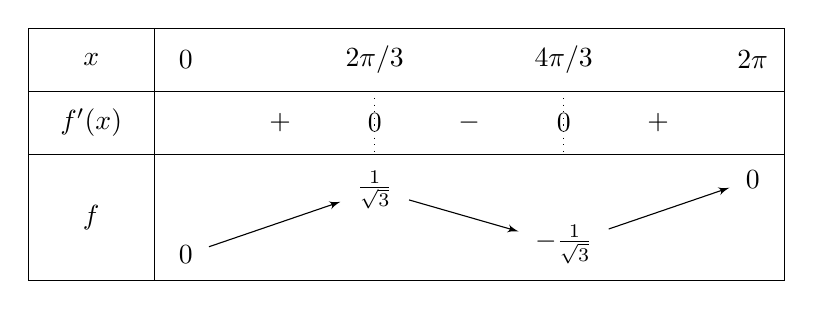
\begin{tikzpicture}[scale=0.8]
   \tkzTabInit{$x$ / 1 , $f'(x)$ / 1, $f$ / 2}{$0$, $2\pi /3$, $4\pi /3$, $2\pi$}
   \tkzTabLine{, +,z,-,z,+,  }
   \tkzTabVar{-/$0$,+/$\frac{1}{\sqrt{3}}$,-/$-\frac{1}{\sqrt{3}}$, +/$0$}
\end{tikzpicture}
\end{center}
\end{solution}




\begin{exercise}Montrer que pour tout réel $x\geqslant 0$, on a $x\geqslant \sin(x)$.\end{exercise}

\begin{solution}Pour tout réel $x\geqslant 0$, on pose $f(x)=x-\sin(x)$. $f$ est dérivable sur $\mathbb{R}_+$ et pour tout réel $x\geqslant 0$, \\$f'(x)=1-\cos(x) \geqslant 0$. $f$ est donc croissante sur $ \mathbb{R}_+$.\\ Ainsi, pour tout réel $x \geqslant0$, $f(x) \geqslant f(0)$, soit $x-\sin(x) \geqslant 0$ et donc $x\geqslant \sin(x)$.\end{solution}




\begin{exercise}Pour tout réel $x$, on pose $f(x)=\cos\left(\e^{-x^2}\right)$.
\begin{enumerate}
\item Déterminer, si elles existent, les limites de $f$ en $+\infty$ et en $-\infty$.
\item Justifier que $f$ est dérivable sur $\mathbb{R}$ et que calculer sa dérivée.
\item Montrer que pour tout réel $x$, $0\leqslant \e^{-x^2} \leqslant 1$.
\item En déduire que pour tout réel $x$, $\sin(\e^{-x^2})\geqslant 0$.
\item En déduire le tableau de variations de $f$.
\end{enumerate}\end{exercise}

\begin{solution}\hspace{0pt}
\begin{enumerate}
\item On sait que $\displaystyle\lim_{x\to +\infty}-x^2 = -\infty$, $\displaystyle\lim_{X\to -\infty}\e^X=0$ et $\displaystyle\lim_{Y\to 0}\cos(x)=1$. Par composition de limite, $\displaystyle\lim_{x\to +\infty}f(x)=1$. De même, $\displaystyle\lim_{x\to -\infty}f(x)=1$.
\vskip5pt
\item $f$ est la composée de fonctions dérivables sur $\mathbb{R}$, elle est donc également dérivable sur $\mathbb{R}$. De plus, pour tout réel $x$, $f'(x)=2x\e^{-x^2}\sin(\e^{-x^2})$.
\vskip5pt
\item D'une part, pour tout réel $x$, $\e^{-x^2}\geqslant 0$. Par ailleurs, pour tout réel $x$, $-x^2 \leqslant 0$ et, par croissance de l'exponentielle sur $\mathbb{R}$, $\e^{-x^2} \leqslant \e^0$ soit $\e^{-x^2} \leqslant 1$.
\vskip5pt
\item Pour tout réel $x$, $0\leqslant \e^{-x^2} \leqslant 1$. Or, la fonction $\sin$ est croissante sur $[0;1]$. Ainsi, pour tout réel $x$, $\sin(0)\leqslant \sin(\e^{-x^2}) \leqslant \sin(1)$ et en particulier, $\sin(\e^{-x^2})\geqslant 0$.
\vskip5pt
\item Pour tout réel $x$, $f'(x)$ est donc du signe de $x$.

\begin{center}
	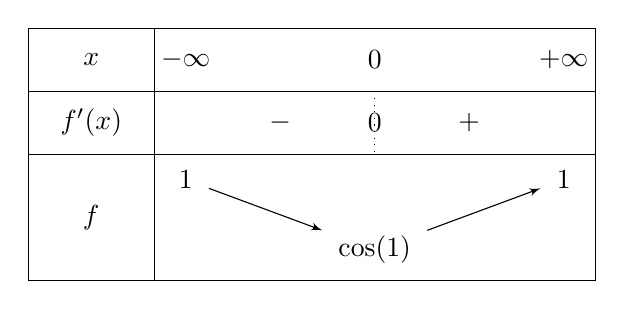
\begin{tikzpicture}[scale=0.8]
   \tkzTabInit{$x$ / 1 , $f'(x)$ / 1, $f$ / 2}{$-\infty$, $0$, $+\infty$}
   \tkzTabLine{, -,z,+,  }
   \tkzTabVar{+/$1$,-/$\cos(1)$, +/$1$}
\end{tikzpicture}
\end{center}

\end{enumerate}\end{solution}




\begin{exercise}Soit $f$ la fonction définie pour tout $x \in \left[-\dfrac{\pi}{2},\dfrac{\pi}{2}\right]$ par $f(x)=x-\sin(x)$.
\begin{enumerate}
\item Montrer que $f$ est strictement croissante sur $\left[-\dfrac{\pi}{2},\dfrac{\pi}{2}\right]$.
\item En déduire que l'équation $\sin(x)=x$ possède une unique solution dans l'intervalle $\left[-\dfrac{\pi}{2},\dfrac{\pi}{2}\right]$. Quelle est-elle ?
\end{enumerate}
On considère la suite $(u_n)$ définie par $u_0=1$ et pour tout entier naturel $n$, $u_{n+1}=\sin(u_n)$.
\begin{enumerate}
\setcounter{enumi}{2}
\item Montrer que pour tout entier naturel $n$, $0 \leqslant u_n \leqslant \dfrac{\pi}{2}$ et que la suite $(u_n)$ est décroissante.
\item En déduire que la suite $(u_n)$ converge. Quelle est sa limite ?
\end{enumerate}\end{exercise}

\begin{solution}\hspace{0pt}
\begin{enumerate}
\item $f$ est dérivable sur $\left[-\dfrac{\pi}{2},\dfrac{\pi}{2}\right]$ et pour tout réel $x$ de cet intervalle, $f'(x)=1-\cos(x) \geqslant 0$ car $\cos(x) \leqslant 1$. Par ailleurs, $f'$ s'annule uniquement en $0$. $f$ est donc strictement croissante sur $\left[-\dfrac{\pi}{2},\dfrac{\pi}{2}\right]$.
\vskip5pt
\item On a $f\left(-\dfrac{\pi}{2}\right)=-\dfrac{\pi}{2}+1 \leqslant 0$ et $f\left(\dfrac{\pi}{2}\right)=\dfrac{\pi}{2}-1 \geqslant 0$. Par ailleurs, $f$ est continue sur  $\left[-\dfrac{\pi}{2},\dfrac{\pi}{2}\right]$. 

D'après le théorème des valeurs intermédiaires, l'équation $f(x)=0$ possède une solution sur cet intervalle. 

De plus, la fonction $f$ étant strictement croissante sur  $\left[-\dfrac{\pi}{2},\dfrac{\pi}{2}\right]$, cette solution est unique. 

Or, $f(0)=0$. $0$ est donc l'unique solution sur  $\left[-\dfrac{\pi}{2},\dfrac{\pi}{2}\right]$ de l'équation $x-\sin(x)=0$, soit $\sin(x)=x$. 
\vskip5pt
\item Pour tout entier naturel $n$, on pose $P(n)$ : « $0 \leqslant u_{n+1} \leqslant u_n \leqslant \dfrac{\pi}{2}$ ».
\begin{itemize}
\item On a $u_0=1$ et $u_1=\sin(1)\leqslant 1$. On a bien $0 \leqslant u_{1} \leqslant u_0 \leqslant \dfrac{\pi}{2}$. $P(0)$ est vraie.
\item Soit $n\in\mathbb{N}$ tel que $P(n)$ est vraie. On a alors $0 \leqslant u_{n+1} \leqslant u_n \leqslant \dfrac{\pi}{2}$. En appliquant la fonction sinus qui est croissante sur $\left[0;\dfrac{\pi}{2}\right]$, on a alors $\sin(0) \leqslant \sin(u_{n+1}) \leqslant \sin(u_n) \leqslant \sin\left(\dfrac{\pi}{2}\right)$. Or, $\sin\left(\dfrac{\pi}{2}\right)=1 \leqslant \dfrac{\pi}{2}$. On a donc bien $0 \leqslant u_{n+2} \leqslant u_{n+1} \leqslant \dfrac{\pi}{2}$.
\item Par récurrence, $P(n)$ est vraie pour tout entier naturel $n$.
\end{itemize}
\vskip5pt
\item La suite $(u_n)$ est décroissante et minorée, elle est donc convergente, de limite $\ell \in \left[0;\dfrac{\pi}{2}\right]$. La fonction sinus étant continue sur cet intervalle, on a alors $\sin(\ell)=\ell$ et donc $\ell=0$ d'après la question 2.
\end{enumerate}\end{solution}




\begin{exercise}Pour tout réel $x>0$, on pose $f(x)=\dfrac{x}{2}\left(\sin(\ln x)-\cos(\ln x)\right)$ et $g(x)=\sin(\ln x)$.\\ Montrer que $f$ est une primitive de $g$ sur $]0;+\infty[$.\end{exercise}

\begin{solution}Pour tout réel $x>0$, posons $u(x)=\sin(\ln(x))$ et $v(x)=\cos(\ln(x))$. $u$ et $v$ sont dérivables et pour tout réel $x>0$, $u'(x)=\dfrac{\cos(\ln(x))}{x}$ et $v'(x)=-\dfrac{\sin(\ln(x))}{x}$. Ainsi, pour tout réel $x>0$,
\[f'(x)=\dfrac{1}{2}(\sin(\ln x)-\cos(\ln x))+\dfrac{x}{2}\left(\dfrac{\cos(\ln(x))}{x} -\left(-\dfrac{\sin(\ln(x))}{x}\right)\right)=\sin(\ln(x)).\]
$f$ est une primitive de $g$ sur $]0;+\infty[$.

\end{solution}




\begin{exercise}On admet que les fonctions suivantes sont continues sur $\mathbb{R}$. Donner une primitive de ces fonctions.
\renewcommand{\arraystretch}{1}

\begin{tabularx}{\linewidth}{XX}
$f_1:x\mapsto \cos(3x)-2\sin(5x)$
& $f_2:x\mapsto \cos(x)-\sin(x)$ \\
 $f_3:x \mapsto 2x\cos(x^2)$
& $f_4:x \mapsto\sin(x)\cos(x)$ \\
\end{tabularx}
\end{exercise}

\begin{solution}

Une primitive de $f_1:x\mapsto \cos(3x)-2\sin(5x)$ est $F_1:x \mapsto \dfrac{1}{3}\sin(3x)+\dfrac{2}{5}\cos(5x)$.

Une primitive de $f_2:x\mapsto \cos(x)-\sin(x)$ est $F_2:x \mapsto \sin(x) + \cos(x)$.

Pour tout réel $x$, on pose $u(x)=x^2$. On a alors $f_3 = u'\cos(u)$, une primitive de $f_3$ est donc $\sin(u)$ soit $x\mapsto \sin(x^2)$.

Pour tout réel $x$, on pose $u(x)=\sin(x)$. On a alors $f_4=u'u = \dfrac{1}{2} (2u'u)$.\\ Une primitive de $f_4$ est donc $\dfrac{u^2}{2}$ soit $x\mapsto \dfrac{\sin(x)^2}{2}$.

\end{solution}



\begin{exercise}Calculer les intégrales suivantes

\begin{tabularx}{\linewidth}{XXX}
a. $\displaystyle\int_0^{\pi} \cos(x)\dx$ & b. $\displaystyle\int_0^{\pi /4} \sin(x)\dx$ & c. $\displaystyle\int_0^{\pi / 6} \sin(2x)\dx$ \\
d. $\displaystyle\int_0^{\pi} \cos(x)\sin(x)^3\dx$ & e. $\displaystyle\int_0^{\sqrt{\pi}}x\cos(2x^2)$ & f. $\displaystyle\int_0^{\pi/4} \dfrac{\sin(x)}{1-\sin(x)^2}\dx$
\end{tabularx}

\end{exercise}


\begin{solution}Calculer les intégrales suivantes

\textbf{a.} $\displaystyle\int_0^{\pi} \cos(x)\dx = [\sin(x)]_0^{\pi}=\sin(\pi)-\sin(0)=0-0=0$.

\textbf{b.} $\displaystyle\int_0^{\pi /4} \sin(x)\dx = [-\cos(x)]_0^{\pi /4}=-\cos\left(\dfrac{\pi}{4}\right)-(-\cos(0))=-\dfrac{\sqrt{2}}{2}+1=\dfrac{2-\sqrt{2}}{2}$.

\textbf{c.} $\displaystyle\int_0^{\pi / 6} \sin(2x)\dx = \left[-\dfrac{\cos(2x)}{2}\right]_0^{\pi/6} = -\dfrac{\cos\left(\frac{\pi}{3}\right)}{2}-\left(-\dfrac{\cos(0)}{2}\right)=-\dfrac{1}{4}+\dfrac{1}{2}=\dfrac{1}{4}$.

\textbf{d.} Pour tout réel $x$, on pose $u(x)=\sin(x)$. On a alors $\cos(x)\sin(x)^3 = u'(x) \times u(x)^3 = \dfrac{1}{4} \times 4u'(x)u(x)^3$. Une primitive de $x\mapsto \cos(x)\sin(x)^3$ est donc $x\mapsto \dfrac{\sin(x)^4}{4}$. \\ Ainsi, $\displaystyle\int_0^{\pi} \cos(x)\sin(x)^3\dx = \left[\dfrac{\sin(x)^4}{4}\right]_0^{\pi}=0-0=0$.

\textbf{e.} Pour tout réel $x$, on pose $u(x)=2x^2$. On a alors $x\cos(2x^2) = \dfrac{1}{4}u'(x)\cos(u(x))$. \\Une primitive de $x\mapsto x\cos(2x^2)$ est donc $x\mapsto \dfrac{\sin(2x^2)}{4}$. \\ Ainsi, $\displaystyle\int_0^{\sqrt{\pi}}x\cos(2x^2) = \left[\dfrac{\sin(2x^2)}{4}\right]_0^{\sqrt{\pi}}= \dfrac{\sin(2\pi)}{4}-\dfrac{\sin(0)}{4}=0-0=0$.

\textbf{f.} Pour tout réel $x\in \left[0;\dfrac{\pi}{4}\right]$, $\dfrac{\sin(x)}{1-\sin(x)^2}=\dfrac{\sin(x)}{\cos(x)^2} = -\dfrac{u'(x)}{u(x)^2}$ en posant $u(x)=\cos(x)$. \\ Une primitive de $x\mapsto \dfrac{\sin(x)}{1-\sin(x)^2}$ sur $\left[0;\dfrac{\pi}{4}\right]$ est donc $x\mapsto \dfrac{1}{\cos(x)}$.\\ Ainsi, $\displaystyle\int_0^{\pi/4} \dfrac{\sin(x)}{1-\sin(x)^2}\dx=\left[\dfrac{1}{\cos(x)}\right]_0^{\pi/4}=\dfrac{1}{\cos(\pi/4)}-\dfrac{1}{\cos(0)}=\sqrt{2}-1$.

\end{solution}




\begin{exercise}À l'aide d'une intégration par parties, déterminer $\displaystyle \int _{0}^{\pi /2} x\cos (x) \dx$.\end{exercise}

\begin{solution}Pour tout réel $x$, on pose $u(x)=x$ on cherche $v$ tel que $v'(x)=\cos(x)$ : on prend donc $v:x\mapsto \sin(x)$. D'après la formule d'intégrations par parties, $\displaystyle \int _{0}^{\pi /2} uv' (x) \dx = [uv]_0^{\pi/2}-\displaystyle \int _{0}^{\pi /2} u'v(x) \dx$.Ainsi, 
\[\displaystyle \int _{0}^{\pi /2} x\cos (x) \dx = [x\sin(x)]_0^{\pi/2}-\displaystyle \int _{0}^{\pi /2}\sin(x)\dx=\dfrac{\pi}{2}-0-[-\cos(x)]_0^{\pi/2}=\dfrac{\pi}{2}-(-0-(-1))=\dfrac{\pi}{2}-1.\]
\end{solution}



\begin{exercise}A l'aide de deux intégrations par parties successives, déterminer $\displaystyle \int _{0}^{\pi /2} \e^x\cos (x) \dx$.\newpage \end{exercise}

\begin{solution}Notons $I=\displaystyle \int _{0}^{\pi /2} \e^x\cos (x) \dx$.

Pour tout réel $x$, on pose $u(x)=\e^x$ on cherche $v$ tel que $v'(x)=\cos(x)$ : on prend donc $v:x\mapsto \sin(x)$. D'après la formule d'intégrations par parties, $\displaystyle \int _{0}^{\pi /2} uv' (x) \dx = [uv]_0^{\pi/2}-\displaystyle \int _{0}^{\pi /2} u'v(x) \dx$.

Ainsi, $\displaystyle \int _{0}^{\pi /2} \e^x\cos (x) \dx = [\e^x\sin(x)]_0^{\pi/2}-\displaystyle \int _{0}^{\pi /2}\e^x\sin(x)\dx=\e^{\pi/2}-\displaystyle \int _{0}^{\pi /2}\e^x\sin(x)\dx$.

Cherchons alors à calculer $\displaystyle \int _{0}^{\pi /2}\e^x\sin(x)\dx$. 

Pour tout réel $x$, on pose $u(x)=\e^x$ on cherche $v$ tel que $v'(x)=\sin(x)$ : on prend donc $v:x\mapsto -\cos(x)$. \\ D'après la formule d'intégrations par parties, $\displaystyle \int _{0}^{\pi /2} uv' (x) \dx = [uv]_0^{\pi/2}-\displaystyle \int _{0}^{\pi /2} u'v(x) \dx$.

Ainsi, $\displaystyle \int _{0}^{\pi /2} \e^x\cos (x) \dx = [-\e^x\cos(x)]_0^{\pi/2}-\displaystyle \int _{0}^{\pi /2}(-\e^x\cos(x))\dx=1+I$.

Ainsi, en reprenant la première IPP, on a $I=\e^{\pi/2}-(1+I)$ et donc $2I=\e^{\pi/2}-1$ et finalement, $I=\dfrac{\e^{\pi/2}-1}{2}$.\end{solution}



\begin{exercise}[subtitle={(Guyane 2018)}]Un publicitaire souhaite imprimer le logo ci-dessous sur un T-shirt : 

\begin{center}
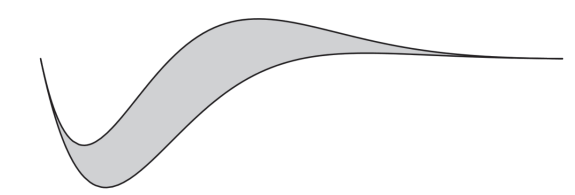
\includegraphics[scale=0.5]{guyane2018}
\end{center}

Il dessine ce logo à l'aide des courbes de deux fonctions$f$ et $g$ définies sur $\mathbb{R}$ par :
\[f(x)=\e^{-x}(-\cos(x)+\sin(x)+1)\quad\text{et}\quad g(x)=-\e^{-x}\cos(x).\]
On admet que les fonctions $f$ et $g$ sont dérivables sur $\mathbb{R}$.

\paragraph{Partie A : Étude de la fonction $f$}

\begin{enumerate}
\item Justifier que pour tout $x\in\mathbb{R}$,
\[-\e^{-x} \leqslant f(x) \leqslant 3\e^{-x}.\]
\item En déduire la limite de $f$ en $+\infty$.
\item Démontrer que, pour tout réel $x$,
\[f'(x)=\e^{-x}(2\cos(x)-1).\]
\item Déterminer le signe de $f'(x)$ pour $x$ appartenant à l'intervalle $[-\pi ; \pi]$ et en déduire les variations de $f$ sur cet intervalle.
\end{enumerate}

\paragraph{Partie B : Aire du logo}

On note $\mathcal{C}_f$ et $\mathcal{C}_g$ les représentations graphiques des fonctions $f$ et $g$ dans un repère orthonormé $(O, \vec i, \vec j)$. Le logo correspond au domaine délimité par la courbe $\mathcal{C}_f$, la courbe $\mathcal{C}_g$ ainsi que les droites d'équation $x=-\dfrac{\pi}{2}$ et $x=\dfrac{3\pi}{2}$.

\begin{center}
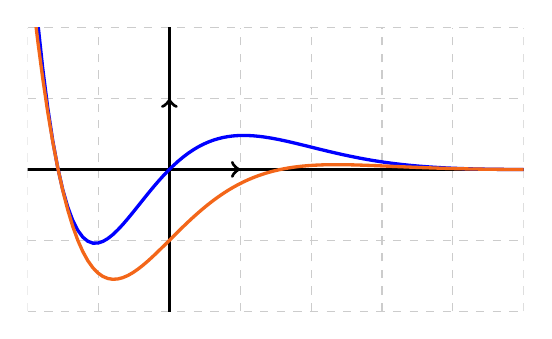
\begin{tikzpicture}[scale=0.9]
\clip (-2,-2) rectangle (5,2);
\draw [thin, dashed, gray!40] (-2,-2) grid (5,2);
\draw [thick] (-6,0)--(9,0);
\draw [thick] (0,-6)--(0,9);
\draw [very thick, ->] (0,0)--(1,0);
\draw [very thick, ->] (0,0)--(0,1);
\draw [blue, very thick,domain=-2:5,samples=100] plot (\x,{exp(-\x)*(-cos(deg(\x))+sin(deg(\x))+1)});
\draw [ocre, very thick,domain=-2:5,samples=100] plot (\x,{-exp(-\x)*cos(deg(\x))});

\end{tikzpicture}
\end{center}

\begin{enumerate}
\item Calculer $f(x)-g(x)$ pour tout réel $x$.
\item En déduire que la courbe de $f$ est toujours au dessus de la courbe de $g$.
\item Soit $H$ la fonction définie pour tout réel $x$ par  $H(x)=\left(-\dfrac{\cos(x)}{2}-\dfrac{ \sin(x)}{2}-1\right)\e^{-x}$. 

Montrer que $H$ est une primitive de la fonction  $x\mapsto (\sin(x)+1)\e^{-x}$ sur $\mathbb{R}$.
\item En déduire l'aire du logo en unité d'aires.
\end{enumerate}

\end{exercise}

\begin{solution}

\paragraph{Partie A : Étude de la fonction $f$}

\begin{enumerate}
\item Pour tout réel $x$, $-1 \leqslant \sin(x) \leqslant $ et $-1\leqslant -\cos(x) \leqslant 1$. En ajoutant ces inégalités puis en ajoutant 1 à chauqe membre, on a que pour tout réel $x$, $-1 \leqslant -\cos(x)+\sin(x)+1 \leqslant 3$, puis, en multipliant par $\e^{-x}$ qui est positif, $-\e^{-x} \leqslant f(x) \leqslant 3\e^{-x}$.
\item On a $\displaystyle\lim_{x \to + \infty}-\e^{-x}=\displaystyle\lim_{x \to + \infty}3\e^{-x}=0$. \\Ainsi, d'après le théorème d'encadrement, $\displaystyle\lim_{x \to + \infty}f(x)$ existe et vaut 0.
\item Pour tout réel $x$, $f'(x)=-\e^{-x}(-\cos(x)+\sin(x)+1)+\e^{-x}(\sin(x)+\cos(x))=\e^{-x}(2\cos(x)-1)$.
\item Sur $[-\pi ; \pi]$, $f'$ est du signe de $2\cos(x)-1$.\\ Or, sur cet intervalle, $2\cos(x)-1\geqslant 0$ ssi $\cos(x)\geqslant \dfrac{1}{2}$ soit $x\in\left[-\dfrac{\pi}{3};\dfrac{\pi}{3}\right]$.

\begin{center}
	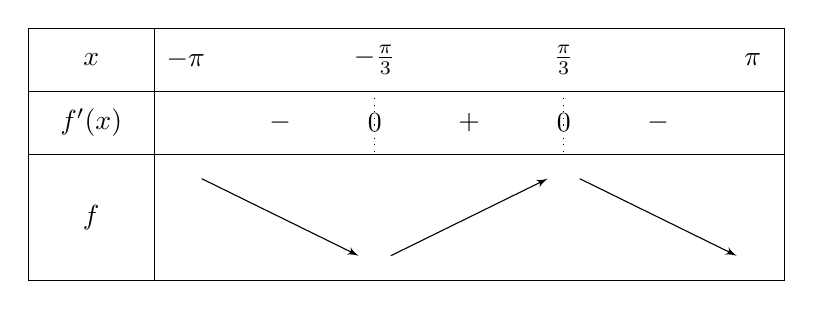
\begin{tikzpicture}[scale=0.8]
   \tkzTabInit{$x$ / 1 , $f'(x)$ / 1, $f$ / 2}{$-\pi$, $-\frac{\pi}{3}$, $\frac{\pi}{3}$, $\pi$}
   \tkzTabLine{, -,z,+,z,-  }
   \tkzTabVar{+/$ $,-/$ $, +/$ $,-/$ $}
\end{tikzpicture}
\end{center}

\end{enumerate}

\paragraph{Partie B : Aire du logo}

\begin{enumerate}
\item Pour tout réel $x$, $f(x)-g(x)=\e^{-x}(\sin(x)+1)$.
\item Pour tout réel $x$, $\e^{-x}>0$ et $\sin(x)+1 \geqslant 0$. Ainsi, pour tout réel $x$, $f(x)-g(x)\geqslant 0$ : la courbe de $f$ est toujours au dessus de la courbe de $g$.
\item Pour tout réel $x$,
\[H'(x)=\left(\dfrac{\sin(x)}{2}-\dfrac{\cos(x)}{2}\right)\e^{-x}+\left(-\dfrac{\cos(x)}{2}-\dfrac{ \sin(x)}{2}-1\right) \times(-\e^{-x}).\]
Ainsi,
\[H'(x)=\e^{-x}\left(\dfrac{\sin(x)}{2}-\dfrac{\cos(x)}{2}-\left(-\dfrac{\cos(x)}{2}-\dfrac{ \sin(x)}{2}-1\right) \right)=(\sin(x)+1)\e^{-x}.\]
 $H$ est une primitive de la fonction  $x\mapsto (\sin(x)+1)\e^{-x}$ sur $\mathbb{R}$.
\item L'aire du logo en unité d'aires vaut $\displaystyle\int_{-\pi/2}^{3\pi/2}(f(x)-g(x))$. \\ Or, pour tout réel $x$, $f(x)-g(x)=(\sin(x)+1)\e^{-x}$. Une primitive de $f-g$ est $H$. 

Ainsi, $\displaystyle\int_{-\pi/2}^{3\pi/2}(f(x)-g(x)) = \left[H(x)\right]_{-\pi/2}^{3\pi/2} \simeq 2,4$. L'aire du logo est d'environ 2,4 unités d'aire.
\end{enumerate}
\newpage
\end{solution}

\begin{exercise}[subtitle={(Centres étrangers 2024)}]

On considère les équations différentielles $(E)\; : \; y'=y-\cos(x)-3\sin(x)$ et $(E_0)\; : \; y'=y$.

\begin{enumerate}
\item Déterminer toutes les solutions de l'équation $(E_0)$.
\item On considère la fonction $h:x\mapsto 2\cos(x)+\sin(x)$, que l'on admet définie et dérivable sur $\R$. \\Montrer que $h$ est solution de l'équation différentielle $(E)$.
\item Soit $f$ une fonction définie et dérivable sur $\mathbb{R}$. \\Montrer que $f$ est solution de $(E)$ si et seulement si $f-h$ est solution de $(E_0)$.
\item En déduire toutes les solutions de l'équation différentielle $(E)$.
\item Déterminer l'unique solution $g$ de $(E)$ telle que $g(0)=0$.
\end{enumerate}

\end{exercise}

\begin{solution}\hspace{0pt}

\begin{enumerate}
\item Les solutions de $(E_0)$ sont les fonctions $x\mapsto C\e^x$, pour $C$ réel.
\item Pour tout réel $x$, on a $f'(x)=-2\sin(x)+\cos(x)$ et \[h(x)-\cos(x)-3\sin(x)=2\cos(x)+\sin(x)-\cos(x)-3\sin(x)=-2\sin(x)+\cos(x)=h'(x).\] Ainsi, $h$ est bien solution de $(E)$.
\item Puisque $h$ est solution de $(E)$, on a $h'=h-\cos(x)-3\sin(x)$ et donc $-\cos(x)-3\sin(x)=h-h'$.

On a $f$ solution de $(E)$ si et seulement si $f'=f-\cos(x)-3\sin(x)=f-(h-h')$ si et seulement si $f'-h'=f-h$ si et seulement si $(f-h)'=f-h$.

 Ainsi, $f$ est solution de $(E)$ si et seulement si $f-h$ est solution de $(E_0)$.
\item Les solutions de $(E)$ sont les fonctions $x\mapsto C\e^x+2\cos(x)+\sin(x)$, pour $C$ réel.
\item On cherche $C$ tel que $C\e^0+2\cos(0)+\sin(0)=0$. On a donc $C+2=0$ et donc $C=-2$. 

Ainsi, pour tout réel $x$, $g(x)=-2\e^x+2\cos(x)+\sin(x)$.
\end{enumerate}

\end{solution}

\begin{exercise}[subtitle={(Amérique du Nord 2024)}]

Pour tout entier naturel $n$, on considère les intégrales suivantes :
\[I_n = \displaystyle\int_0^{\pi}\e^{-nx}\sin(x)\dx \qquad J_n=\displaystyle\int_0^{\pi}\e^{-nx}\cos(x)\dx\]

\begin{enumerate}
\item Calculer $I_0$
\vskip10pt
\item \begin{enumerate}
\item Justifier que pour tout entier naturel $n$, on a $I_n \geqslant 0$.
\item Justifier que pour tout entier naturel $n$, on a $I_{n+1}-I_n \leqslant 0$.
\item Déduire des deux questions précédentes que la suite $(I_n)$ converge.\end{enumerate}
\vskip10pt
\item \begin{enumerate} \item Justifier que pour tout entier naturel $n$, on a $I_n \leqslant \displaystyle\int_0^{\pi} \e^{-nx}\dx$
\item Montrer que pour tout entier naturel $n\geqslant 1$, on a :
\[\displaystyle\int_0^{\pi}\e^{-nx}\dx=\dfrac{1-\e^{-n\pi}}{n}\]
\item Déduire des deux questions précédentes la limite de la suite $(I_n)$. \end{enumerate}
\vskip10pt
\item \begin{enumerate} \item Rappeler la formule d'intégration par parties.
\item En intégrant par parties l'intégrale $I_n$ de deux façons différents, établir les deux relations suivantes, pour tout entier naturel $n\geqslant 1$.
\[I_n=1+\e^{-n\pi}-nJ_n \quad\text{et}\quad I_n=\dfrac{1}{n}J_n\]
\item En déduire que, pour tout entier naturel $n\geqslant 1$, on a $I_n=\dfrac{1+\e^{-n\pi}}{n^2+1}$\end{enumerate}
\item On souhaite obtenir le rang $n$ à partir duquel la suite $(I_n)$ devient inférieure à 0,1. Recopier et compléter la cinquième ligne du script Python ci-dessous avec la commande appropriée.
\begin{lstlisting}[language=python]
from math import *
def seuil():
	n = 0
	I = 2
	...
		n = n + 1
		I = (1 + exp(-n * pi))/(n*n + 1)
	return n

\end{lstlisting}
\end{enumerate}
\newpage
\end{exercise}

\begin{solution}\hspace{0pt}


\begin{enumerate}
\item On a $I_0=\displaystyle\int_0^{\pi}\sin(x)\dx$. 

Une primitive de $\sin$ étant $-\cos$, on a $I_0=[-\cos(x)]_0^{\pi}=-\cos(\pi)-(-\cos(0))=-(-1)-(-1)=2$.
\item \begin{enumerate}
\vskip5pt
\item Pour tout entier naturel $n$ et pour tout réel $x \in [0; \pi]$, $\e^{-nx}>0$ et $\sin(x)>0$. 

Ainsi, $\e^{-nx}\sin(x)>0$ et donc $I_n \geqslant 0$.
\vskip5pt
\item Pour tout entier naturel $n$ et pour tout réel $x$, $\e^{-(n+1)x}\sin(x)-\e^{-nx}\sin(x)=\e^{-nx}\sin(x) \times(\e^{-x}-1)$. Or, pour tout réel $x\in[0;\pi]$, $\e^{-x} \leqslant 1$ et donc $\e^{-x}-1 \leqslant 0$.

Ainsi, pour tout $x \in [0;\pi]$, on a $\e^{-(n+1)x}\sin(x)-\e^{-nx}\sin(x)\leqslant 0$. 

Alors $\displaystyle\int_0^{\pi}(\e^{-(n+1)x}\sin(x)-\e^{-nx}\sin(x))\dx\leqslant 0$ soit $\displaystyle\int_0^{\pi}\e^{-(n+1)x}\sin(x)\dx-\int_0^{\pi}\e^{-nx}\sin(x)\dx\leqslant 0$. 

Finalement, $I_{n+1}-I_n \leqslant 0$.
\vskip5pt
\item D'après la question 2a, la suite $(I_n)$ est minorée. \\D'après la question 2b, la suite $(I_n)$ est décroissante.\\ Ainsi, la suite $(I_n)$ converge.\end{enumerate}

\item \begin{enumerate}
\item Pour tout réel $x$, $\sin(x)\leqslant 1$. 

Ainsi, pour tout entier naturel $n$ et pour tout réel $x\in[0;\pi]$, $\e^{-nx}\sin(x) \leqslant \e^{-nx}$. 

En intégrant cette inégalité, on a donc $I_n \leqslant \displaystyle\int_0^{\pi} \e^{-nx}\dx$.
\vskip5pt
\item Une primitive de $x\mapsto \e^{-nx}$ est $x\mapsto -\dfrac{\e^{-nx}}{n}$. Ainsi, $\displaystyle\int_0^{\pi} \e^{-nx}\dx=\left[ -\dfrac{\e^{-nx}}{n}\right]_0^{\pi}=\dfrac{1-\e^{-n\pi}}{n}$.
\vskip5pt
\item Ainsi, pour tout entier naturel $n$, $0 \leqslant I_n \leqslant \dfrac{1-\e^{-n\pi}}{n}$. Or, $\displaystyle\lim_{n \to +\infty} \dfrac{1-\e^{-n\pi}}{n} = \displaystyle\lim_{n \to + \infty}0=0$. 

D'après le théorème d'encadrement, on a donc $\displaystyle\lim_{n \to +\infty}I_n=0$.
\end{enumerate}
\vskip5pt
\item \begin{enumerate}

\item On rappelle que $I_n=\displaystyle\int_0^{\pi}\e^{-nx}\sin(x)\dx$.

D'une part, pour tout réel $x\in[0;\pi]$, on pose $\left\{\begin{array}{ll}u(x)=\e^{-nx} & u'(x)=-n\e^{-nx} \\ v(x)= -\cos(x) & v'(x)=\sin(x)\end{array}\right.$

D'après la formule d'intégration par parties,
\[I_n=\left[-\e^{-nx}\cos(x)\right]_0^{\pi}-\displaystyle\int_0^{\pi}(-n\e^{-nx}) \times (-\cos(x))\dx=1+\e^{-n\pi}-n\displaystyle\int_0^{\pi}\e^{-nx}\cos(x)\dx = 1+\e^{-n\pi}-nJ_n.\]

D'autre part, pour tout réel $x\in[0;\pi]$, on pose $\left\{\begin{array}{ll}w(x)=\sin(x) & w'(x)= \cos(x) \\ p(x)=-\dfrac{\e^{-nx}}{n} & p'(x)=\e^{-nx}\end{array}\right.$

D'après la formule d'intégration par parties,
\[I_n = \left[-\dfrac{\e^{-nx}}{n}\sin(x)\right]_0^{\pi}-\displaystyle\int_{0}^{\pi}\left(-\dfrac{\e^{-nx}}{n}\right)\cos(x)\dx=0-0+\dfrac{1}{n}\displaystyle\int_0^{\pi}\e^{-nx}\cos(x)\dx=\dfrac{1}{n}J_n.\]

\item On a donc $I_n=\dfrac{1}{n}J_n$ donc $J_n=nI_n$. Or, $I_n=1+\e^{-n\pi}-nJ_n=1+\e^{-n\pi}-n^2I_n$. 

Ainsi, $(n^2+1)I_n=1+\e^{-n\pi}$ et finalement $I_n=\dfrac{1+\e^{-n\pi}}{1+n^2}$.\end{enumerate}

\item 
\begin{lstlisting}[language=python]
from math import *
def seuil():
	n = 0
	I = 2
	while I >= 0.1:
		n = n+1
		I = (1+exp(-n*pi))/(n*n+1)
	return n
\end{lstlisting}

\end{enumerate}

\end{solution}


\section*{Pour aller plus loin...}

\begin{exercise}[subtitle={(Fonction tangente)}]Pour $x$ tel que $\cos(x)\neq 0$, on appelle tangente de $x$, noté $\tan (x)$, le réel :
\[ \tan (x) = \dfrac{\sin (x)}{\cos (x)}.\]
\textbf{Partie A : Quelques valeurs}
\begin{enumerate}
\item Que valent $\tan \left( \dfrac{\pi}{4} \right)$, $\tan \left( \dfrac{2\pi}{3} \right)$ et $\tan \left( \dfrac{-3\pi}{4} \right)$ ?
\item On considère un réel $x \in \left] -\pi ; \dfrac{-\pi}{2} \right[$ tel que $\sin (x) = -\dfrac{11}{61}$.
\begin{enumerate}
\item Que vaut $\cos (x)$ ?
\item Que vaut $\tan (x)$ ?
\end{enumerate}
\item Résoudre l'inéquation $\tan(x) \leqslant 0$ sur $\left]-\dfrac{\pi}{2};\dfrac{\pi}{2}\right[$.
\end{enumerate}
\textbf{Partie B : Un peu d'étude de la tangente}\\
On considère la fonction $x\mapsto \tan (x)$, définie sur $\left]-\dfrac{\pi}{2};\dfrac{\pi}{2}\right[$.
\begin{enumerate}
\item Montrer que la fonction $\tan$ est impaire.
\item Montrer que pour tout réel $x\in\left]-\dfrac{\pi}{2};\dfrac{\pi}{2}\right[$, $1+(\tan(x))^2=\dfrac{1}{(\cos(x))^2}$.
\item Justifier que $\tan$ est dérivable sur $\left]-\dfrac{\pi}{2};\dfrac{\pi}{2}\right[$ et que $\tan$ est solution de l'équation différentielle $y'=1+y^2$ sur cet intervalle.
\item En déduire le sens de variation de la fonction $\tan$ sur $\left]-\dfrac{\pi}{2};\dfrac{\pi}{2}\right[$.
\item Justifier que $\tan$ est deux fois dérivable sur $\left]-\dfrac{\pi}{2};\dfrac{\pi}{2}\right[$ et déterminer les intervalles de $\left]-\dfrac{\pi}{2};\dfrac{\pi}{2}\right[$ sur lesquels cette fonction est convexe.
\item Tracer la courbe représentative de la fonction $\tan$ sur $\left]-\dfrac{\pi}{2};\dfrac{\pi}{2}\right[$ dans un repère orthogonal.
\item Déterminer l'unique primitive de $\tan$ sur $\left[0;\dfrac{\pi}{2}\right]$ qui vaut 0 en 0.
\end{enumerate}
\end{exercise}

\begin{solution}
\textbf{Partie A : Quelques valeurs}
\begin{enumerate}
\item $\tan \left( \dfrac{\pi}{4} \right) = \dfrac{\sin\left(\frac{\pi}{4}\right)}{\cos\left(\frac{\pi}{4}\right)}=\dfrac{\frac{\sqrt{2}}{2}}{\frac{\sqrt{2}}{2}}=1 \qquad \tan \left( \dfrac{2\pi}{3} \right)=\dfrac{\sin\left(\frac{2\pi}{3}\right)}{\cos\left(\frac{2\pi}{3}\right)}=\dfrac{\frac{\sqrt{3}}{2}}{-\frac{1}{2}}=-\sqrt{3}$. \\ $\tan \left( \dfrac{-3\pi}{4} \right)=\dfrac{\sin\left(\frac{-3\pi}{4}\right)}{\cos\left(\frac{-3\pi}{4}\right)}=\dfrac{-\frac{\sqrt{2}}{2}}{-\frac{\sqrt{2}}{2}}=1$ .
\vskip5pt
\item Puisque $x \in \left] -\pi ; \dfrac{-\pi}{2} \right[$, alors $\cos(x)\leqslant 0$. De plus, $\cos(x)^2+\sin(x)^2=1$. \\ Ainsi, $\cos(x)^2=1-\dfrac{121}{3721}=\dfrac{3600}{3721}$ et donc $\cos(x)=-\sqrt{\dfrac{3600}{3721}}=-\dfrac{60}{61}$ Ainsi, $\tan(x)=\dfrac{-\frac{11}{61}}{-\frac{60}{61}}=\dfrac{11}{60}$.
\vskip5pt
\item Soit $x \in \left]-\dfrac{\pi}{2};\dfrac{\pi}{2}\right[$. Alors $\cos(x)>0$, $\tan(x)$ est donc du signe de $\sin(x)$.\\ Ainsi, $\tan(x)\leqslant 0$ si et seulement si $x\in \left]-\dfrac{\pi}{2};0\right]$.
\end{enumerate}

\textbf{Partie B : Un peu d'étude de la tangente}
\begin{enumerate}
\item L'intervalle $\left]-\dfrac{\pi}{2};\dfrac{\pi}{2}\right[$ est centré en 0.\\ De plus, pour tout réel $x$ de cet intervalle, $\tan(-x)=\dfrac{\sin(-x)}{\cos(-x)}=\dfrac{-\sin(x)}{\cos(x)}=-\tan(x)$.\\ La fonction $\tan$ est impaire.
\vskip5pt
\item Pour tout réel $x\in\left]-\dfrac{\pi}{2};\dfrac{\pi}{2}\right[$, $1+(\tan(x))^2=1+\dfrac{\sin(x)^2}{\cos(x)^2}=\dfrac{\cos(x)^2+\sin(x)^2}{(\cos(x))^2}=\dfrac{1}{\cos(x)^2}$.
\vskip5pt
\item $\tan$ est dérivable sur $\left]-\dfrac{\pi}{2};\dfrac{\pi}{2}\right[$ comme quotient de fonctions dérivables dont le dénominateur ne s'annule pas sur cet intervalle. De plus, pour tout réel $x\in\left]-\dfrac{\pi}{2};\dfrac{\pi}{2}\right[$, \[\tan'(x)=\dfrac{\cos(x)\cos(x)-\sin(x) \times (-\sin(x))}{\cos(x)^2}=\dfrac{\cos(x)^2+\sin(x)^2}{\cos(x)^2}=\dfrac{1}{\cos(x)^2}=1+\tan(x)^2\] $\tan$ est solution de l'équation différentielle $y'=1+y^2$ sur $\left]-\dfrac{\pi}{2};\dfrac{\pi}{2}\right[$.
\vskip5pt
\item Pour tout réel $x\in\left]-\dfrac{\pi}{2};\dfrac{\pi}{2}\right[$, $\tan'(x)\geqslant 0$. $\tan$ est donc croissante sur $\left]-\dfrac{\pi}{2};\dfrac{\pi}{2}\right[$.
\vskip5pt
\item La fonction $\tan' : x\mapsto \dfrac{1}{\cos(x)^2}$ est dérivable sur $\left]-\dfrac{\pi}{2};\dfrac{\pi}{2}\right[$ et pour tout réel $x$ de cet intervalle, on a $\tan''(x)=-\dfrac{-\sin(x)}{\cos(x)^4}=\dfrac{\sin(x)}{\cos(x)^4}$. $\tan''$ est donc du signe de $\sin$. Or, la fonction sinus est négative sur $\left]-\dfrac{\pi}{2};0\right]$ et positive sur  $\left[0;\dfrac{\pi}{2}\right[$. $\tan$ est donc concave sur $\left]-\dfrac{\pi}{2};0\right]$ et convexe sur $\left[0;\dfrac{\pi}{2}\right[$.
\vskip5pt
\item On trace la courbe représentative de la fonction $\tan$ sur $\left]-\dfrac{\pi}{2};\dfrac{\pi}{2}\right[$ dans un repère orthogonal.

\begin{center}
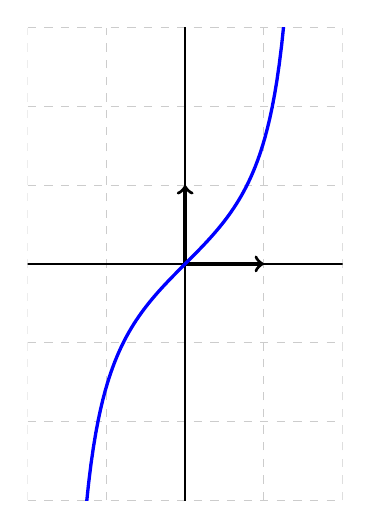
\begin{tikzpicture}[scale=1]
\clip (-2,-3) rectangle (2,3);
\draw [thin, dashed, gray!40] (-2,-3) grid (2,3);
\draw [thick] (-6,0)--(9,0);
\draw [thick] (0,-6)--(0,9);
\draw [very thick, ->] (0,0)--(1,0);
\draw [very thick, ->] (0,0)--(0,1);
\draw [blue, very thick,domain=-1.5:1.5,samples=100] plot (\x,{tan(deg(\x))});

\end{tikzpicture}
\end{center}

\item Pour tout $x\in\left]-\dfrac{\pi}{2};\dfrac{\pi}{2}\right[$, $\tan(x)=-\dfrac{\cos'(x)}{\cos(x)}$. De plus, sur $\left]-\dfrac{\pi}{2};\dfrac{\pi}{2}\right[$, $\cos(x)>0$. 

Les primitives de $\tan$ sur $\left]-\dfrac{\pi}{2};\dfrac{\pi}{2}\right[$ sont donc les fonctions $x\mapsto -\ln(\cos(x)) +C$, où $C$ est un réel. 

Or, $-\ln(\cos(0))=-\ln(1)=0$. L'unique primitive de $\tan$ sur $\left[0;\dfrac{\pi}{2}\right]$ qui vaut 0 en 0 est donc la fonction $x\mapsto -\ln(\cos(x))$.
\end{enumerate}
\end{solution}




\begin{exercise}[subtitle={(Tension efficace)}]
Soit $f$ une fonction continue sur un intervalle [a;b]. On appelle valeur efficace de la fonction $f$ est égale à la racine carrée de la valeur moyenne de $f^2$ sur l'intervalle $[a,b]$.

En électricité, la valeur efficace d'un courant ou d'une tension variables au cours du temps correspond à la valeur d'un courant continu ou d'une tension continue qui produirait un échauffement identique dans une résistance.

Dans le cas d'un régime sinusoïdal, l'intensité du courant est donnée par une fonction $i : t \mapsto I_{max}\sin(\omega t)$, où $I_{max}$ est un réel positif et $\omega$ désigne la pulsation du signal. L'intervalle considérée est l'intervalle $\left[0;\dfrac{2\pi}{\omega}\right]$;

\begin{enumerate}
\item Montrer que la fonction $x\mapsto \dfrac{I_{max}^2}{2}\left(x-\dfrac{\sin(\omega x)\cos(\omega x)}{\omega}\right)$ est une primitive de $i^2$ sur $[0;2\pi]$.
\item En déduire que l'intensité efficace d'un tel courant vaut $\dfrac{I_{max}}{\sqrt{2}}$.
\end{enumerate}\newpage \end{exercise}

\begin{solution}
On considère la fonction $F:x\mapsto \dfrac{I_{max}^2}{2}\left(x-\dfrac{\sin(\omega x)\cos(\omega x)}{\omega}\right)$. $f$ est dérivable et pour tout réel $x$, 
\[F'(x)=\dfrac{I_{max}^2}{2}\left(1-\dfrac{\omega \cos(\omega x) \cos (\omega x)- \omega \sin( \omega x) \sin (\omega x)}{\omega}\right)=\dfrac{I_{max}^2}{2}\left(1-\cos^2(\omega x)+\sin^2(\omega x)\right).\]

En rappelant que pour tout réel $X$, $\cos^2(X)+\sin^2(X)=1$, on obtient alors
\[ F'(x) = \dfrac{I_{max}^2}{2}(\sin^2(\omega x)+\sin^2(\omega x))=I_{max}^2\sin^2(\omega x)=i^2(x).\]

$F$ est une primitive de $i^2$ sur $[0;2\pi]$. L'intensité efficace d'un tel courant vaut
\[ \sqrt{ \dfrac{1}{\frac{2\pi}{\omega}-0}\int_{0}^{\frac{2\pi}{\omega}} i^2(x)\dx} = \dfrac{\sqrt{\omega}}{\sqrt{2\pi}}\sqrt{F\left(\frac{2\pi}{\omega}\right)-F(0)}.\]
Or, $F\left(\frac{2\pi}{\omega}\right)=\dfrac{\pi I_{max}^2}{\omega}$ et $F(0)=0$. Ainsi, l'intensité efficace vaut $\dfrac{\sqrt{\omega}}{\sqrt {2\pi}} \times \sqrt{\dfrac{\pi I_{max}^2}{\omega}}=\dfrac{I_{max}}{\sqrt{2}}$.
 \end{solution}
 
 

\begin{exercise}[subtitle={(Fonction arcsinus)}]

L'objectif de l'exercice est de présenter la réciproque de la fonction sinus sur l'intervalle $\left[-\dfrac{\pi}{2};\dfrac{\pi}{2}\right]$.

\begin{enumerate}
\item Soit $x\in [-1;1]$. Justifier que l'équation $\sin(a)=x$, d'inconnue réelle $a$, possède exactement une solution sur l'intervalle $\left[-\dfrac{\pi}{2};\dfrac{\pi}{2}\right]$. 
\end{enumerate}
Cette solution sera notée $\arcsin (x)$. On définit alors la fonction $\arcsin$ comme étant la fonction qui à un réel $x\in[-1;1]$ associe l'unique de l'équation $\sin(a)=x$ d'inconnue $a$ \textbf{sur l'intervalle $\left[-\dfrac{\pi}{2};\dfrac{\pi}{2}\right]$}.
\vskip10pt
\begin{enumerate}
\setcounter{enumi}{1}
\item Soit $x\in [-1;1]$. Que vaut $\sin(\arcsin(x))$ ? Que vaut $\arcsin(\sin(\pi))$ ?
\vskip10pt
\item Montrer que pour tout $x\in[-1;1]$, $\cos(\arcsin(x))=\sqrt{1-x^2}$.
\vskip10pt
\item On admet que la fonction $x\mapsto \arcsin (x)$ est dérivable sur $]-1;1[$. En utilisant les deux questions précédentes, montrer que pour tout $x\in ]-1;1[$
\[\arcsin'(x)=\dfrac{1}{\sqrt{1-x^2}}.\]
\item A l'aide d'une intégration par parties, déterminer $\displaystyle\int_0^{1/2} \arcsin(x) \dx$.
\end{enumerate}
\end{exercise}


\begin{solution}\hspace{0pt}
\begin{enumerate}
\item La fonction sinus est continue et strictement croissante sur l'intervalle $\left[-\dfrac{\pi}{2};\dfrac{\pi}{2}\right]$. \\ Par ailleurs, $\sin\left(-\dfrac{\pi}{2}\right)=-1$ et $\sin\left(\dfrac{\pi}{2}\right)=1$. Ainsi, d'après le théorème des valeurs intermédiaires appliqué aux fonctions strictement monotones, l'équation $\sin(a)=x$ admet une unique solution sur $\left[-\dfrac{\pi}{2};\dfrac{\pi}{2}\right]$ pour tout réel $x$ dans l'intervalle $[-1;1]$.
\vskip5pt
\item Soit $x\in [-1;1]$. Par définition, $\sin(\arcsin(x))=x$. 

En revanche $\arcsin(\sin(\pi))=\arcsin(0)=0$. 

En particulier, on n'a pas $\arcsin(\sin(x))=x$ pour tout réel $x$ : cette égalité n'est vraie que sur $\left[-\dfrac{\pi}{2};\dfrac{\pi}{2}\right]$.
\vskip5pt
\item Pour tout $x\in[-1;1]$, $\cos^2(\arcsin(x))+\sin^2(\arcsin(x))=1$ d'où $\cos^2(\arcsin(x))+x^2=1$ et donc  \\ $\cos^2(\arcsin(x))=1-x^2$. Par ailleurs, puisque $\arcsin(x)\in \left[-\dfrac{\pi}{2};\dfrac{\pi}{2}\right]$, on a $\cos(\arcsin(x))\geqslant 0$. 

On en déduit que $\cos(\arcsin(x))=\sqrt{1-x^2}$.
\vskip5pt
\item On admet que la fonction $x\mapsto \arcsin (x)$ est dérivable sur $]-1;1[$. 

Pour tout $x\in]-1,1[$, on a $\sin(\arcsin(x))=x$. En dérivant, on en déduit que pour tout $x\in]-1;1[$, $\arcsin'(x) \times \cos(\arcsin(x))=1,$ soit $\arcsin'(x)=\dfrac{1}{\cos(\arcsin(x))}=\dfrac{1}{\sqrt{1-x^2}}$.
\vskip5pt
\item Pour tout réel $x\in \left[0;\dfrac{1}{2}\right]$, on pose $u(x)=\arcsin(x)$ et $v(x)=x$. On a alors $u'(x)=\dfrac{1}{\sqrt{1-x^2}}$ et $v'(x)=1$. Par intégration par parties,
\[\displaystyle\int_0^{1/2} \arcsin(x) \dx = \left[x\arcsin(x)\right]_0^{1/2}-\int_0^{1/2}\dfrac{x}{\sqrt{1-x^2}}\dx.\]
D'une part, $\left[x\arcsin(x)\right]_0^{1/2} = \dfrac{1}{2}\arcsin\left(\dfrac{1}{2}\right)-0=\dfrac{1}{2}\times \dfrac{\pi}{6}=\dfrac{\pi}{12}$. 

Par ailleurs, si l'on pose, pour tout réel $x$, $w(x)=1-x^2$, alors $w'(x)=-2x$. \\ On a alors $-\dfrac{x}{\sqrt{1-x^2}}=\dfrac{-2x}{2\sqrt{1-x^2}}=\dfrac{w'(x)}{2\sqrt{w(x)}}$. \\ Ainsi, une primitive de la fonction $x\mapsto \dfrac{-x}{\sqrt{1-x^2}}$ sur $\left[0;\dfrac{1}{2}\right]$ est la fonction $x \mapsto \sqrt{1-x^2}$. Il en vient
\[-\int_0^{1/2}\dfrac{x}{\sqrt{1-x^2}}\dx=[\sqrt{1-x^2}]_0^{1/2}=\sqrt{1-\left(\dfrac{1}{2}\right)^2}-\sqrt{1-0^2}=\dfrac{\sqrt{3}}{2}-1.\]

Finalement,
\[\displaystyle\int_0^{1/2} \arcsin(x) \dx = \dfrac{\pi}{12}+\dfrac{\sqrt{3}}{2}-1.\]
Oui, il faut parfois s'attendre à ce genre de résultat pas franchement sexy.

\end{enumerate}
\newpage
\end{solution}




\begin{exercise}[subtitle={(Intégrales de Wallis)}]

Pour tout entier naturel $n$, on pose $W_n = \displaystyle\int_0^{\pi/2} \sin^n(x) \dx$.

\paragraph{Partie A : Convergence de la suite $(W_n)$}

\begin{enumerate}
\item Calculer $W_0$ et $W_1$.
\item Justifier que pour tout entier naturel $n$, $W_n >0$.
\item Montrer que la suite $(W_n)$ est décroissante. 
\item Que peut-on en déduire sur la suite $(W_n)$ ?
\end{enumerate}

\paragraph{Partie B : Calcul du terme général}

\begin{enumerate}
\item Montrer que pour tout entier naturel $n$, on a $W_{n+2}=\dfrac{n+1}{n+2}W_n$. \\
On pourra utiliser une intégration par parties en utilisant la fonction $u :x \mapsto \sin^{n+1}(x)$ et en déterminant une fonction $v$ telle que pour tout réel $x\in\left[0;\dfrac{\pi}{2}\right]$, $v'(x)=\sin(x)$.
\item En déduire que pour tout entier naturel $p$, on a
\[W_{2p}=\dfrac{\pi}{2}\dfrac{(2p)!}{(2^pp!)^2}\quad \text{et}\quad W_{2p+1}=\dfrac{(2^pp!)^2}{(2p+1)!}.\]
\end{enumerate}

\paragraph{Partie C : Étude asymptotique}

Pour tout entier naturel $n$, on pose $J_n=(n+1)W_{n+1}W_n$.
\begin{enumerate}
\item En s'aidant de la question \textbf{B1}, montrer que la suite $(J_n)$ est constante. Quelle est sa valeur ?
\item En s'aidant des questions \textbf{B1} et \textbf{A3}, montrer que pour tout entier naturel $n$, on a
\[\dfrac{n+1}{n+2} \leqslant \dfrac{W_{n+1}}{W_n}\leqslant 1.\]
\item Déduire des questions précédentes que $\displaystyle\lim_{n \to + \infty} \dfrac{2}{\pi}n W_n^2=1$.
\end{enumerate}


\end{exercise}

\begin{solution}


\paragraph{Partie A : Convergence de la suite $(W_n)$}

\begin{enumerate}
\item On a $W_0 = \int_0^{\pi/2} 1 \dx = \dfrac{\pi}{2}$ et $W_n = \int_0^{\pi/2} \sin^1(x) \dx=[-\cos(x)]_0^{\pi/2}=0-(-1)=1$.
\item Pour tout $x\in \left[0;\dfrac{\pi}{2}\right]$, $\sin(x)\geqslant 0$. Il en vient que, pour tout entier naturel $n$, $W_n\geqslant 0$. De plus, pour tout $x \in \left[\dfrac{\pi}{6};\dfrac{\pi}{2}\right]$, $\sin(x)\geqslant \dfrac{1}{2}$ et donc 
\[W_n \geqslant \int_{\pi/6}^{\pi/2} \sin^n(x) \dx \geqslant \int_{\pi/6}^{\pi/2} \left(\dfrac{1}{2}\right)^n \dx = \dfrac{\pi}{3}\left(\dfrac{1}{2}\right)^n >0.\]
\item Pour tout entier naturel $n$,
\[W_{n+1}-W_n=\int_0^{\pi/2} (\sin^{n+1}(x)-\sin^n(x)) \dx = \int_0^{\pi/2} \sin^n(x)(\sin(x)-1) \dx .\]
Or, pour tout $x\in  \left[0;\dfrac{\pi}{2}\right]$, $\sin^n(x)\geqslant 1$ et $\sin(x)-1 \leqslant 0$. Il en vient que $W_{n+1}-W_n \leqslant 0$. La suite $(W_n)$ est donc décroissante.
\item La suite $(W_n)$ est décroissante et minorée par 0, elle est donc convergente.
\end{enumerate}

\paragraph{Partie B : Calcul du terme général}

\begin{enumerate}
\item Soit $n$ un entier naturel. 

On considère la fonction $u :x \mapsto \sin^{n+1}(x)$ et $v:x\mapsto -\cos(x)$, définies sur $\left[0;\dfrac{\pi}{2}\right]$. 

Pour tout réel $x$ de cet intervalle, on a alors $u'(x)=(n+1)\cos(x)\sin^n(x)$ et $v'(x)=\sin(x)$. 

Par intégration par parties, on obtient alors
\[W_{n+2}\int_0^{\pi/2} \sin^{n+2}(x)\dx = \int_0^{\pi/2} \sin^{n+1}(x) \times \sin(x) \dx = \left[-\sin^{n+1}(x)\cos(x)\right]_0^{\pi/2}+(n+1)\int_0^{\pi/2}\cos^2(x)\sin^n(x)\dx.\]

D'une part, $\left[-\sin^{n+1}(x)\cos(x)\right]_0^{\pi/2}=0$. Par ailleurs, pour tout réel $x$, $\cos^2(x)=1-\sin^2(x)$. Ainsi,
\[W_{n+2}=(n+1)\int_0^{\pi/2}(1-\sin^2(x))\sin^n(x)\dx = (n+1)\int_0^{\pi/2}(\sin^n(x)-\sin^{n+2}(x))\dx = (n+1)(W_n-W_{n+2}).\]

On a donc $W_{n+2}=(n+1)W_n-(n+1)W_{n+2}$ et donc $(n+2)W_{n+2}=(n+1)W_n$.

Finalement, on retrouve bien $W_{n+2}=\dfrac{n+1}{n+2}W_n$.

\item Pour tout entier naturel $p$, on a alors
\[W_{2p}=\dfrac{2p-1}{2p}W_{2p-2}=\dfrac{2p-1}{2p}\dfrac{2p-3}{2p-2}W_{2p-4}= \dots =\dfrac{2p-1}{2p} \times \dfrac{2p-3}{2p-2} \times \dots \times \dfrac{3}{4} \times \dfrac{1}{2} W_0.\]

Or, en factorisant chaque terme par 2, on a \[2p(2p-2)(2p-4)...\times 4 \times 2=2^p \times p(p-1)(p-2)... \times 1 = 2^pp!.\]

On retrouve au numérateur le produit de tous les nombres impairs de 1 à $2p-1$ et au dénominateur le produit de tous les nombres pairs de 2 à $2p-2$.
En multipliant numérateur et dénominateur par le produit $2p(2p-2)(2p-4)...\times 4 \times 2$, on complète alors le produit du numérateur : on multiplie tous les nombres de $1$ à $2p$ : il s'agit tout simplement de $(2p)!$.

Finalement, pour tout entier naturel $p$, $W_{2p}=\dfrac{(2p)!}{(2^pp)^2}W_0 = \dfrac{\pi}{2}\dfrac{(2p)!}{(2^pp!)^2}$. 

De même, pour tout entier naturel $p$,
\[W_{2p+1}=\dfrac{2p}{2p+1}W_{2p-1}=\dfrac{2p}{2p+1}\dfrac{2p-2}{2p-1}W_{2p-3}= \dots =\dfrac{2p}{2p+1} \times \dfrac{2p-2}{2p-1} \times \dots \times \dfrac{2}{3} \times W_1.\]

En multipliant encore une fois le numérateur et le dénominateur par $2p(2p-2)(2p-4)...\times 4 \times 2$, on a alors $W_{2p+1}=\dfrac{(2^pp!)^2}{(2p+1)!}W_1=\dfrac{(2^pp!)^2}{(2p+1)!}$.

Si vous savez manipuler la notation produit $\prod$, n'hésitez pas à l'utiliser pour résoudre cet exercice.

\end{enumerate}

\paragraph{Partie C : Étude asymptotique}

Pour tout entier naturel $n$, on pose $J_n=(n+1)W_{n+1}W_n$.
\begin{enumerate}
\item Pour tout entier naturel $n$, $J_{n+1}-J_n = (n+2)W_{n+2}W_{n+1}-(n+1)W_{n+1}W_n$. 

Or, d'après la question \textbf{B1}, $W_{n+2}=\dfrac{n+1}{n+2}W_n$. 

Ainsi, $J_{n+1}-J_n = (n+2)\dfrac{n+1}{n+2}W_nW_{n+1}-(n+1)W_{n+1}W_n=0$.

Or, $J_0=W_1W_0=\dfrac{\pi}{2}$. La suite $(J_n)$ est donc constante égale à $\dfrac{\pi}{2}$.

\item D'une part, la suite $(W_n)$ est décroissante et positive. Ainsi, pour tout entier naturel $n$, $\dfrac{W_{n+1}}{W_n} \leqslant 1$. 

Par ailleurs, toujours par décroissance de la suite $(W_n)$, pour tout entier naturel $n$, $W_{n+1} \geqslant W_{n+2}$ et donc, en utilisant la question \textbf{B1},  $W_{n+1} \geqslant \dfrac{n+1}{n+2}W_n$ d'où $\dfrac{n+1}{n+2} \leqslant \dfrac{W_{n+1}}{W_n}$.

\item Pour tout entier naturel non nul $n$, $nW_nW_{n-1}=\dfrac{\pi}{2}$ d'où $W_{n-1}=\dfrac{\pi}{2nW_n}$. 

Or, pour tout entier naturel non nul $n$, $\dfrac{n}{n+1} \leqslant \dfrac{W_n}{W_{n-1}} \leqslant 1$.

 Ainsi, en remplaçant $W_{n-1}$ dans cette inégalité, on a $\dfrac{n}{n+1} \leqslant   \dfrac{2}{\pi}n W_n^2 \leqslant 1$.

Or, $\displaystyle\lim_{n\to+\infty}\dfrac{n}{n+1}=\displaystyle\lim_{n\to+\infty}=1$. D'après le théorème d'encadrement, $\displaystyle\lim_{n \to + \infty} \dfrac{2}{\pi}n W_n^2$ existe et vaut 1.
\end{enumerate}
\end{solution}




\chapter{Corrigés}


\printsolutions[headings={false} ]

\end{document}